% !Mode:: "Tex:UTF-8"
\chapter{解空间上估计的混淆算法}
\label{chap:5}
第三、四章研究了SAT问题求解中CNF公式的隐私保护,也即SAT问题输入数据的保护。本章把保护的范围进一步扩展到输出数据,
研究可同时保护SAT问题输入和输出数据隐私的
方法。
该方法基于解空间上估计的混淆算法和解恢复算法。
通过该混淆算法,CNF公式被变换为具有不同电路结构的新公式,并且该公式的解空间为原公式的解空间的上估计。原始公式的解可通过映射方法从混淆后公式的解中恢复。
理论分析证明了算法的正确性和有效性。
理论分析和实验表明混淆算法具有多项式复杂度,而解恢复算法仅线性复杂度;
在ISCAS89 测试集上的实验表明,该混淆算法引入了可接受的SAT 求解开销。
\section{引言}
命题可满足\upcite{SATtheory}(简称SAT)问题求解在软硬件验证\upcite{HardwareSAT,softwareSAT}和密码学\upcite{cryptoSAT} 等领域得到广泛应用。
近年来,软硬件规模的日益扩大,服务于软硬件验证和密码破解的SAT问题规模也随之急剧膨胀。
另一方面,云计算、网格计算等依托开放环境的计算模式可以根据应用规模提供弹性的计算资源,
将复杂的SAT问题外包到云或网格环境下成为一种有吸引的解决方案\upcite{Nordugrid,CloudSMT,OneSpin}。

但是,对安全的担忧阻碍了大多数用户将其关键应用部署到开放环境中运行。
由于网格计算是由松散耦合的高端计算设施组成\upcite{Nordugrid},网格环境下恶意计算节点的威胁是可预见的\cite{HV-grid};
在云计算环境下,虽然云硬件平台提供商及其基础设施(虚拟层)是可被信赖,在其上运行的虚拟机却不总是可以信赖的。
文献\upcite{AMI}指出,著名的云计算提供商亚马逊的EC2受到了虚拟机影像滥用的困扰,
被污染虚拟机映像会迅速扩散到整个社区;
而文献\upcite{InformationLeakageofCloud}则指出了处于同一台物理机器上的虚拟机之间攻击的可能性。

%These facts show that input and output data of SAT problem may be exposed to untrusted third party,
%who may inspect valuable information from these data.
%For example, SAT program originated from verification may suffer from leakage of privacy, such as circuit structure information.
%Works carried out by Roy\upcite{csRoy} and Fu \upcite{csFu} suggest the possibility of extracting circuit information from CNF formula.
%Furthermore, Du\upcite{HV-grid} called solution of hard SAT problem generating from cryptograph etc as high-value rare events,
%and point out that the solution of SAT problem should also be treated as privacy,
%because it may be leaked to third party by hoarding participants.
%Moreover, the SAT solver deployed in grid or Cloud may also be compromised by adversary,
%who may compel SAT solver to return incorrect result to  mislead verification.
这些事实指出,外包到云计算或网格环境下的SAT问题,
其输入和输出数据可能会被未授权的第三方访问。
这些潜在的威胁者可能会从这些数据中获取有价值的信息。
例如,来源于软硬件验证的SAT问题,可能遭受硬件结构信息泄露的问题。
Roy\upcite{csRoy}和Fu\upcite{csFu}的工作指出了从CNF公式中抽取电路结构信息的可能性。
而针对计算结果的完整性,Du\upcite{HV-grid}归纳了开放计算环境下存在的三类威胁:懒惰计算者、奇货可居者、恶意欺骗者。懒惰计算者不给或是给出不完整的结果;恶意欺骗者给出错误结果,奇货可居的计算参与者会计算出正确结果但会因利益问题将结果泄露给第三方。
结果验证技术[7][30]可以有效制止懒惰者和恶意欺骗者的行为,但对制止奇货可居者却并不奏效,Du\upcite{HV-grid}指出将SAT 问题求解由显式稀有事件(ORE)转化为隐式稀有事件(CRE)是解决输出数据隐私的最终之道。
%另一方面,Du\upcite{HV-grid}将某些复杂SAT问题的解称作高价值稀有事件,指出SAT问题的解也应该被视作为隐私,
%如来源于密码破解的SAT问题,恶意计算参与者可能会因利益问题而将其泄露给第三方。

为了解决上述问题,本章给出了一个在保持求解方法不变的前提下,保护SAT 问题外包过程中输入输出隐私方法。
%
%命题可满足\upcite{SATtheory} (简称SAT)问题求解在软硬件验证\upcite{HardwareSAT,softwareSAT}、密码学\cite{cryptoSAT} 等领域得到广泛应用。
%近年来,软硬件规模的日益扩大,服务于软硬件验证、密码破解的SAT问题规模也随之急剧膨胀。
%另一方面,云计算、网格计算等依托开放环境的计算模式可以根据应用规模提供弹性的计算资源,
%将复杂的SAT问题外包到云或网格环境下成为一种有吸引的解决方案\upcite{Nordugrid,CloudSMT,OneSpin}。
%但是,对安全的担忧阻碍了大多数用户将其关键应用部署到grid或云上运行。
%由于网格计算是由松散耦合的高端计算设施组成\upcite{Nordugrid},网格环境下恶意计算节点的威胁是可预见的\cite{HV-grid};
%在云计算环境下,虽然云硬件平台提供商及其基础设施(虚拟层)是可被信赖,在其上运行的虚拟机却不总是可以信赖的,
%文献\upcite{AMI}指出,著名的云计算提供商亚马逊的EC2受到了虚拟机影像滥用的困扰,
%被污染虚拟机映像会迅速扩散到整个社区;
%而文献\upcite{InformationLeakageofCloud}则指出了处于同一台物理机器上的虚拟机之间攻击的可能性。
%这些事实指出,外包到云计算或网格环境下的SAT问题,
%其输入和输出数据可能会被未授权的第三方访问,
%这些潜在的威胁者可能会从这些数据中获取有价值的信息。
%例如,来源于软硬件验证的SAT问题,可能遭受硬件结构信息泄露的问题。
%Roy\upcite{csRoy}和Fu\upcite{csFu}的工作指出了从CNF公式中抽取电路结构信息的可能性。
%另一方面,Du\upcite{HV-grid}将某些复杂SAT问题的解称作高价值稀有事件,指出SAT问题的解也应该被视作为隐私,
%如来源于密码破解的SAT问题,恶意计算参与者可能会因利益问题而将其泄露给第三方。
%最后,部署在网格或云环境下的SAT求解器可能会被迫使返回错误的结果。
%这些威胁将用户置于进退维谷的境地:使用公共的云计算或网格计算基础设施具有很好的性价比,但是却会面临隐私泄露和错误结果的困扰。
%为了解决上述问题,我们给出了一个在保持求解方法不变的前提下,保护SAT 问题外包过程中输入输出隐私方法。
%本文的主要贡献在于:首次提出了结构感知的CNF混淆算法,该算法可以在SAT问题计算外包时保护输入和输出数据的隐私。
%该算法具有以下特点:首先通过混淆,原始CNF公式中的诸如电路结构等敏感信息在混淆后的CNF公式中不再存在。
%第二,混淆后的CNF公式可已使用目前已有的SAT求解器求解;
%第三,原始公式的解可以从上估计混淆后CNF公式的解中恢复,这使得SAT求解器也无法知道确切的解信息;
%最后,混淆算法为多项式复杂度,而解恢复算法仅为线性复杂度,减少了SAT求解的开销。
%本章的结构组织如下。
%第二章介绍了相关的术语;第三章给出了云计算环境下的威胁模型;
%第四章给出了基于混淆的隐私保护SAT求解框架的实现;
%第五章分析了算法的正确性、有效性和算法复杂性;
%第六章介绍了相关工作;
%第七章给出了实验结果;
%第八章总结了本文的工作。
%\section{术语}

\section{问题描述}
\subsection{系统假设}
本章以云计算环境为例来阐述SAT求解外包中可能遇到的安全威胁。
就威胁模型而言,网格计算和云计算类似。
%illustrate possible threats when outsourcing SAT solving,
%since grid is same as Cloud as for threat model.

%In our research, there are two types of Cloud, private Cloud and public Cloud.
%Private Cloud is trusted but has only limited computation power and memory to handle simple computation.
%While public Cloud can provide elastic computation and memory resource to deal with complex computation.
%CNF formula will be generated from netlist or program in private Cloud,
%while SAT solover is deployed in public Cloud to solve the CNF formula and return the solution to the private Cloud.
在我们的研究中,存在两种类型的云:私有云和公共云。私有云是可信的但是计算以及存储能力受限,适合处理简单计算;
公共云可以提供弹性的计算和存储资源,可以承担复杂计算任务。
CNF公式将在私有云中由网表产生,SAT求解器部署在公共云,用于求解CNF公式,并将结果返回给私有云。

% Generating CNF formula from netlist or program will be held in private Cloud.
% While SAT solver is deployed in public Cloud,where SAT solver will receive CNF formula as input,
% and output the solution of CNF formula,then return the result to private Cloud.
%\subsection{攻击模型}

%Algorithms \upcite{csLiequivalency,csOstrowski,csRoy,csFu}
%have been proposed to extract and utilize circuit structure in CNF formula.
%Circuit structure extraction algorithms,
%presented by Roy et al. \upcite{csRoy} and Fu et al.\upcite{csFu},
%are based on subgraph isomorphism and pattern matching technique,
%and can recover lots of circuits from CNF formula.
%These pattern matching or subgraph isomorphism techniques are available freely.
%In public Cloud computing environment, adversary, who has controled VM\upcite{InformationLeakageofCloud,AMI},
%may use these algorithms to recover the circuit structure from the CNF formula.

文献\upcite{csLiequivalency,csOstrowski,csRoy,csFu}
研究了抽取和利用CNF公式中电路结构的方法。
Roy等人\upcite{csRoy}和Fu等人\upcite{csFu}给出了基于子图同构以及模式匹配的电路结构抽取算法,
并能最大限度的恢复出CNF公式中的电路结构。这些技术可能会被潜在的攻击者利用来抽取敏感的电路结构信息。
%As pointed out by literature \upcite{HV-grid}, since solutions to difficult instances of NP-complete problems are rare events,
%with the practical importance of many of these problems, hoarding participants may keep these solutions for economic value.
正如文献\upcite{HV-grid}指出,由于复杂SAT问题的解是稀有事件,且这些解具有很重要的实用价值,恶意的计算参与者可能会保留这些解,来获取经济利益。
%%Therefore both CNF formula and its solutions should  be treated as privacy that should be preserved.
因此,同CNF公式一样,公式的解也应该被当做隐私加以保护。
%As a result,
%in our research,
%we assume there are
%curious and hoarding participants\upcite{HV-grid} in public Cloud.
%That means,
%the participants conduct all the required computations to get solutions of SAT problem;
%But they may try to get information from CNF formula as much as possible,
%such as circuit structure information;
%And if the solution are valuable, they may keep the computation results and leak it to third party.

在我们的研究工作中,假设公共云环境下有“诚实且好奇“的计算参与者。
他们会尽力完成所有的计算任务以便获得CNF公式的解,
但是它们也试图从CNF公式或解中获得他们需要的信息,例如电路结构和解。

\section{系统设计}

\subsection{基于混淆的SAT求解框架}
%When we design the Cloud or grid oriented SAT solving framework, the following four goals are taken into consideration:
结合以上的系统假设,
当我们设计基于云或是网格的SAT求解框架时,将考虑下面四个因素:
%\begin{enumerate}
% \item
%%First,
%As for the portability, current SAT solvers with conflict analysis \upcite{Minisat} are very efficient.
%So we would like to use them directly
%instead of developing new algorithms like \upcite{OBfuscationd-CNFs}.
% \item \label{g2}
%%  Second,
%%As for the stealth,the framework should prevent circuit structure recovering based on pattern matching or subgraph isomorphism;
%As for the stealth\upcite{obfuscationBible}, the framework should be able to prevent circuit structure from being recovered from CNF formula.
%%the framework should prevent accurate solution being known even by the SAT solver.
%\item \label{g3}
%%Third,
%%As for the stealth,the framework should prevent circuit structure recovering based on pattern matching or subgraph isomorphism;
%As for the resilence\upcite{obfuscationBible}, the framework should prevent accurate solution from being known even by the SAT solver, which is deployed in public Cloud.
% \item
%%Fourth,
%As for the cost, the framework should not incur too much overhead.
%\end{enumerate}

\begin{enumerate}
 \item
%First,
可移植性:目前的SAT求解器集成了冲突检测等高效机制,因此我们希望可以将其作为黑盒直接使用,而不是像\upcite{OBfuscationd-CNFs}那样试图使用新的求解算法。
%instead of developing new algorithms like \upcite{OBfuscationd-CNFs}.
 \item \label{g2}
%  Second,
%As for the stealth,the framework should prevent circuit structure recovering based on pattern matching or subgraph isomorphism;
隐形性\upcite{obfuscationBible}:求解框架应该可以保护CNF公式中的电路结构不会被获取。
\item \label{g3}
%Third,
%As for the stealth,the framework should prevent circuit structure recovering based on pattern matching or subgraph isomorphism;
%As for the resilence\upcite{obfuscationBible}, the framework should prevent accurate solution from being known even by the SAT solver, which is deployed in public Cloud.
适应性\upcite{obfuscationBible}:求解框架应能防止包括运行于公共云上的求解器在内的第三方获取真实的求解结果。
 \item
%Fourth,
%As for the cost, the framework should not incur too much overhead.
开销:框架不应该引入太多的开销。
\end{enumerate}
%
%
%According to these goals,
%we present a privacy-preserving SAT solving framework based on CNF formula obfuscation.
%To obfuscate the CNF formula,
%according to SSH rules and CSA strategies described below,
%we embed extra literals into CNF clauses and insert extra clauses into CNF formula.
%The extra literals and part of new clauses are from another CNF formula, which we called Husks formula.
%SSH rules and CSA strategies ensure the original CNF formula to be blended with Husks formula seamless,
%to attain goals  \ref{g2}) and \ref{g3}).
%SSH rules and CSA strategies are described in \textit{\ref{embeded rules})} and \textit{\ref{embeded strategy})}.

根据上述目标,
本章给出了一个输入输出隐私保护的SAT求解框架,该框架基于CNF公式混淆算法。
为了混淆CNF公式,
根据后续章节介绍的SSH规则和CSA策略,
在CNF公式的子句中加入新的文字,并在公式中加入新的子句。
新加入的文字和一部分新的子句来自于另外一个CNF公式,称这个公式为Husks公式。
SSH规则和CSA策略保证原始的CNF公式可以和Husk公式无缝地混合在一起,以达到\ref{g2}) 和 \ref{g3})的要求。
SSH规则和CSA策略将在\textit{\ref{embeded rules})} 和 \textit{\ref{embeded strategy})} 小节中介绍。

%\begin{definition}[Singular Husk formula]\label{Singular-Husk-formula-definition}
%Singular Husk formula is a CNF formula with only one solution,
%and assignments of variables in this solution is non-uniform,
%that is,
%not all 0 or all 1.
%\end{definition}
%
%\begin{definition}[Husks formula]\label{Husks-formula-definition}
%Husks formula is a satisfiable CNF formula with more than one solution,
%and assignments of variables in each of its solutions are non-uniform,
%that is,
%not all 0 or all 1.
%\end{definition}
%
%\begin{definition}[单一Husk公式]\label{Singular-Husk-formula-definition}
%单一Husk公式是仅有一个可满足解的CNF公式,
%并且解中变量的赋值是非特异的,也就是不是全$T$或全$F$。
%\end{definition}

\begin{definition}[Husks公式]\label{Husks-formula-definition}
Husks公式是包含一个以上解的可满足公式,
并且解中变量的赋值是非特异的,也就是不是全$T$或全$F$。
\end{definition}
% \begin{definition}[unique cluster shaped solution]
% unique cluster shaped solutions means, CNF formula $F$ has $m+n$ variables,
% while assignments of n variables are unique in all the solutions of $F$.
% \end{definition}
%Detailed implementation of this framework is shown in Figure \ref{fig_cldSAT}.

框架的详细实现在图 \ref{fig_cldSAT}中给出。在框架下, SAT问题的求解包含了4步。\\
$\textbf{步骤 1}$, GENERATOR 产生一个Husks公式$F_H$和它的一个解$R_H$。\\
$\textbf{步骤 2}$, OBFUSCATOR混淆原始CNF公式$F_C$,并产生一个新的CNF公式$F_O$。\\
$\textbf{步骤 3}$, $F_O$由位于公共云上的SAT求解器求解,并返回结果$S_O$。\\
$\textbf{步骤 4}$, MAPPER和VERIFIER从$S_O$中抽取出$S_C$,并确认$S_C$是$F_C$的解。
\begin{figure}
\footnotesize\centering
\centerline{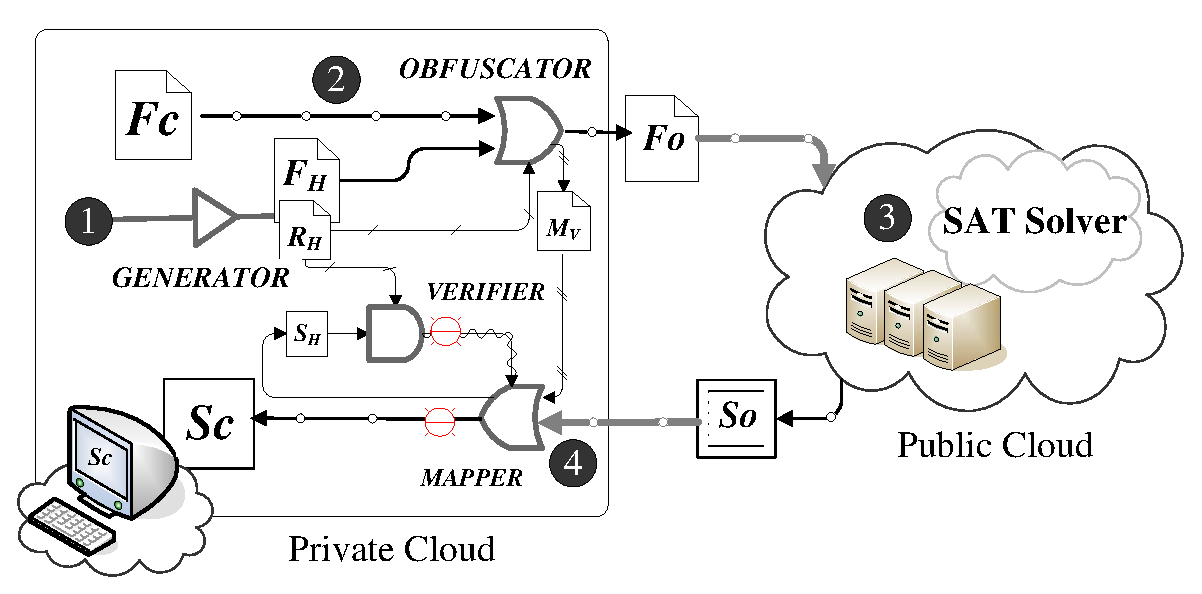
\includegraphics[width=12.2cm]{Visio-cloudsat.eps}}
\caption{输入输出隐私保护的SAT求解框架}
%\caption{Privacy-preserving SAT solving framework based on CNF formula obfuscation.}
\label{fig_cldSAT}
\end{figure}
%In this framework, SAT problem is solved in 4 steps.\\
% \begin{enumerate}
% \item[$\textbf{Step 1,}$]GENERATOR algorithm generates a Husks formula $F_H$ and one of its solution $R_H$.
% \item[$\textbf{Step 2,}$]OBFUSCATOR algorithm obfuscates the Original CNF $F_C$ to obtain a new CNF formula $F_O$.
% \item[$\textbf{Step 3,}$]$F_O$ is solved by SAT Solver deployed in public Cloud, which returns solution $S_O$.
% \item[$\textbf{Step 4,}$]MAPPER and VERIFIER algorithm maps $S_O$ to $S_C$, and check if $F_C$ is satisfied under $S_C$.
% \end{enumerate}%
%$\textbf{Step 1}$, GENERATOR algorithm generates a Husks formula $F_H$ and one of its solution $R_H$.\\
%$\textbf{Step 2}$, OBFUSCATOR algorithm obfuscates the Original CNF $F_C$ to obtain a new CNF formula $F_O$.\\
%$\textbf{Step 3}$, $F_O$ is solved by SAT Solver deployed in public Cloud, which returns solution $S_O$.\\
%$\textbf{Step 4}$, MAPPER and VERIFIER algorithm maps $S_O$ to $S_C$, and check if $F_C$ is satisfied under $S_C$.
% % $\mathbf{Step 1}$, GENERATOR algorithm generates a Husks formula $F_H$ and one of its solution $R_H$.
%
% $\mathbf{Step 2}$, OBFUSCATOR algorithm obfuscates the Original CNF $F_C$ to obtain a new CNF formula $F_O$.
%
% $\mathbf{Step 3}$, $F_O$ is solved by SAT Solver deployed in Cloud, which returns solution $S_O$.
%
% $\mathbf{Step 4}$, MAPPER and VERIFIER algorithm maps $S_O$ to $S_C$,the sulution  of $F_C$, and check if $F_C$ is satisfied under $S_C$.

\textbf{步骤 3}在公共云中运行,其余的步骤在可信的私有云上运行。
%
%The GENERATOR, OBFUSCATOR, MAPPER and VERIFIER algorithms will be described in Subsection \ref{genhusk}, \ref{obfuscating}
%and \ref{mappping} respectively.
GENERATOR, OBFUSCATOR, MAPPER 和 VERIFIER 算法将在 \ref{genhusk}, \ref{obfuscating} 和\ref{mappping}小节中分别介绍。
\subsection{Husks公式的产生}\label{genhusk}

%There are several methods to generate satisfiable CNF formula\upcite{microgenSAT,genSAT}.
%In this paper, Husks formula (in Definition \ref{Husks-formula-definition}) is constructed based on prime factorization method,
%as described in literature\upcite{genSAT}.
%
%GENERATOR algorithm to generate Husks formula is shown in Algorithm \ref{algo2_gen}.

产生可满足CNF公式的算法有多种\upcite{microgenSAT,genSAT}。本文中,定义\ref{Husks-formula-definition}中指出的Husks公式采用质因数的方法构造\upcite{genSAT}。
产生Husks公式的GENERATOR的实现在算法\ref{5:algo2_genSAT}中描述。
%
%\textbf{First},
%given two primes $p_A \neq p_B$ (at line \ref{primenumber}),
%% represented by a binary vector $p_A = <a_1,a_2,\dots,a_n>$, $p_B = <b_1,b_2,\dots,b_n>$,
%we assign $p_A \cdot p_B$ to the output of a multiplier $M$ with constraint $I_1\ne 1$ and  $I_2\ne 1$ (at line \ref{multiplePrime}).
%$I_1$ and $I_2$ are inputs of $M$.
%
%\textbf{Second},
%we convert the multiplier $M$ into CNF formula $Tseitin(M)$ (at line \ref{TseitinPHI}).
\textbf{首先},
给定两个质数$p_A \neq p_B$(第 \ref{primenumber}行),
% represented by a binary vector $p_A = <a_1,a_2,\dots,a_n>$, $p_B = <b_1,b_2,\dots,b_n>$,
将$p_A * p_B$ 赋值给乘法器$M$的输出,并且限制$I_1\ne 1$ and  $I_2\ne 1$ (第\ref{multiplePrime}行)。
其中,$I_1$和$I_2$ 是$M$的输入。

\textbf{第二},
将乘法器$M$编码为CNF公式$Tseitin(M)$(第\ref{TseitinPHI}行)。

为了满足$Tseitin(M)$, $M$的两个输入一定是$\{I_1=p_A,I_2=p_B\}$ 或 $\{I_1=p_B,I_2=p_A\}$,
这就使得$p_A|p_B$或$p_B|p_A$ 为$Tseitin(M)$的两个解。
我们取其中一个为$R_H$。
%
% \begin{procedure}
% \item[input]  NULL
% \item[output] Husks CNF $F_H$ and Husks result $R_H$
% \Begin{
% Generating prime numbers $p_A$ and $p_B$  \; \label{primenumber}
% $\Phi= M(I_1 \neq 1, I_2\neq 1, O=p_A*p_B)$ \;\label{multiplePrime}
% $F_H=Tseitin(\Phi)$ \;\label{TseitinPHI}
% $R_H=p_A\mid p_B$ \;
% }
% \caption{GENERATOR}
% \label{algo2_genSAT}
% \end{procedure}
%Singular Husk formula with unique solution (in Definition \ref{Singular-Husk-formula-definition}) can also be constructed by similar method described in Algorithm \ref{algo2_gen},
%by constraining $p_A\equiv p_B$.
%仅有一个可满足解的单一Husk公式(见定义\ref{Singular-Husk-formula-definition})也可采用算法\ref{5:algo2_genSAT}的方法构造,限制$p_A\equiv p_B$。

构造具有两个以上部分赋值解(见定义\ref{4:Cubic-Husk-formula-definition})的Husk公式也可采用类似的方法。
这里给出一个简单构造方法:以两个质数$P_B$和$P_C$构成的合数替换原有的一个输入$P_B$作为新输入,由构造过程可知,使CNF满足的输入可以是($I_1=P_A$,$I_2=P_B×P_C$)、($I_1=P_B×P_C$,$I_2=P_A$)、($I_1=P_A×P_B$,$I_2=P_C$)、($I_1=P_C$,$I_2=P_A×P_B$)、
($I_ 1=P_A×P_C$,$I_2=P_B$)、($I_1=P_B$,$I_2=P_A×P_C$),这六种组合就构成了该公式的六个解,不妨任取其中四个解,取解中赋值相同的变量集合作为$R_H$;取另外两个解中赋值相同的变量集合作为$S_H$;我们将得到两个部分赋值解,且两个部分赋值解所包含的解个数比例为2:1。使用类似的方法,通过选择合适的合数作为输入并且选择适当的解组合为部分赋值解,我们可以构造解空间不同的Husks公式。


 \begin{algorithm}[t]
 \caption{GENERATOR}
 \label{5:algo2_genSAT}
 \begin{algorithmic}[1]
 \STATE input : NULL;
 \STATE output : Husks CNF $F_H$ and Husks result $R_H$;
 \STATE Generating prime numbers $p_A$ and $p_B$  ; \label{primenumber}
 \STATE $\Phi= M(I_1 \neq 1, I_2\neq 1, O=p_A*p_B)$ ;\label{multiplePrime}
 \STATE $F_H=Tseitin(\Phi)$ ;\label{TseitinPHI}
 \STATE $R_H=p_A\mid p_B$ ;
 \end{algorithmic}
 \end{algorithm}

 \begin{algorithm}[t]
\caption{OBFUSCATOR}
\label{algo_obs}
%\SetAlgoNoLine
\begin{algorithmic}[1]
\STATE input : The original CNF $F_C$, Husks CNF $F_H$, Husks result $R_H$
\STATE output : The obfuscated CNF $F_O$, variable mapping $M$
\STATE $mark(F_C)$;\label{mark}
\FOR{$c\in F_C$}
\IF{$c \in$  Key Clause Set } \label{keyclause}
\STATE     lit =get literal $ \in R_H$;
\STATE     $c=c \cup \neg lit$;\label{rule1}
\STATE     $nc=generate\_new\_clause(c,lit)$;\label{gennewclause}
 \STATE    $F_C=F_C \cup nc$;\label{blendclause1}
\ENDIF
\ENDFOR
\FOR{$ c \in F_C $}
\STATE $averagelen=\frac{\sigma _{c'\in F_C}|c'|}{|F_C|}$ ;
\WHILE{$|c| < averagelen$}
\STATE $lit=$get literal $\in R_H$ ;
\WHILE{$\neg lit \in c$}
\STATE lit=get literal $ \in R_H $ ;
\ENDWHILE
\STATE $c=c \cup \neg lit$;\label{rule1-2}
\ENDWHILE
\STATE $M$ =remap all variable in $F_C\cup F_H$ ;\label{MV}
\STATE $F_O$ =reorder all clause in $F_C\cup F_H$ ; \label{blendclause2}
\ENDFOR
\end{algorithmic}
\end{algorithm}

\begin{algorithm}[t]
\caption{$\mathbf{mark}$ and $\mathbf{generate\_new\_clause}$}
\label{algo_mark}
\begin{algorithmic}[1]
%\SetAlgoNoLine
\STATE $\mathbf{mark}$;
\STATE input : CNF formula $S$;
\STATE output : marked $S$ ;
\FOR{$(C \in S) ~\&~ (|C|\equiv 3)$}
\FOR{$l \in C$ }
\FOR{$(C_1 \in S) ~\&~ (\neg l\in C_1)~ \&~ (|C_1|\equiv 2)$ }
\FOR{$l_1 \in C_1$ }
\IF{$(\neg l_1 \in C)~\&~(l_1\ne l)$}
\STATE $match++$ ;
\ENDIF
\ENDFOR
\ENDFOR
\ENDFOR
\ENDFOR
\IF{$match\equiv 2$}
\STATE mark $l$ as output literal ;
\STATE mark $C$ as Key Clause;
\ENDIF

\STATE $\mathbf{generate\_new\_clause}$;
\STATE input : key clause $C$ in AND2, Husk literal $lit$;
\STATE output : new clause $C_1$;
\STATE $olit$=Getting output literal from $C$ ;
\STATE $C_1= lit \cup \neg olit$ ;\label{rule2}
\end{algorithmic}
\end{algorithm}

\subsection{解空间上估计的混淆}\label{obfuscating}
\subsubsection{CNF公式中的结构}\label{CNF structure5}
%\textbf{Circuit structure in CNF formula}\label{CNF structure5}
%Since we want to protect circuit structure in CNF formula,
%let's first study how the circuit can be recovered from CNF formula.
%Literatures\upcite{csRoy,csFu} have proposed algorithms to recover circuit structure from CNF formula in details.
%Before discussing them, some concepts should be introduced first.
在设计可以防止电路结构信息泄露的混淆算法之前,我们首先开讨论如何从CNF公式中获取电路结构信息。
文献\upcite{csRoy,csFu}给出了从CNF公式中获取电路结构信息的算法细节,在介绍这些算法之前,首先了解算法中用到的概念。
%
%\begin{definition}[CNF signature]
%CNF signature of gate $g$ is its Tseitin encoding $Tseitin(g)$.
%Each clause in CNF signature is called characteristic clause.
%A characteristic clause containing all variables in CNF signature is a \textbf{key clause}.
%Variable corresponding to output of a gate is called \textbf{output variable}.
%\end{definition}
\begin{definition}[CNF标记]
门$g$的CNF标记就是它的Tseitin编码$Tseitin(g)$。
CNF标记中的每个子句称为门的\textbf{特征子句}。
包含门中所有变量的特征子句称为\textbf{关键子句}。
对应于门输出的变量称为\textbf{输出变量}。
\end{definition}

%For AND2 in Equation (\ref{eqn_andinv}),
%$\neg e\vee c$ is a characteristic clause.
%Clause $e\vee \neg c\vee\neg d$ is a key clause.
%$e$ is an output variable.
%
%As metioned in \upcite{csRoy},
%gates with the same characteristic functions will be encoded into the same CNF signature.

公式(\ref{eqn_andinv})中的 AND2门,
$\neg e\vee c$ 是它的一个特征子句,
$e\vee \neg c\vee\neg d$是它的关键子句。
$e$是输出变量。

%As metioned in \upcite{csRoy},
%gates with the same characteristic functions will be encoded into the same CNF signature.

文献\upcite{csRoy}指出,具有相同特征函数的门在同一种规则下都将被编码为相同的CNF标记。
% Some such algorithms\upcite{csRoy,csFu} are based on concept of directed hyper-graph.
%
% \begin{definition}
% [Hypergraph and Directed Hypergraph of CNF]
% A Hypergraph $G=(V,E)$ of a CNF formula $\Sigma$ is
% \begin{enumerate}
%  \item[-] each vertex of $V$ corresponds to a clause of $\Sigma$;
%  \item[-] each edge $(c_1,c_2)\in E$ corresponds to two clauses $c_1$ and $c_2$ containing the same variable or its negation;
%  \item[-] each edge is labeled by the variable;
% \end{enumerate}
% A Directed Hypergraph is a Hypergraph with each endpoint of edge labeled
% by plus when clause contains positive variable,
% or minus when clause contains negative variable.
% \end{definition}
%With these definitions,
%Roy et al. \upcite{csRoy}
%first converts the CNF to an Hypergraph $G$,
%and then matches the CNF signatures of all types of gates in $G$ to recover gates by subgraph isomorphism,
%finally creates a maximal independent set instance to represent the recovered circuit.
%
%Fu et al.\upcite{csFu} presents another algorithm that
%first detects all possible gates with key clause and CNF signature based pattern matching,
%and then constructs a maximum acyclic combinational circuit by selecting a maximum subset of matched gate.
%
%Potential attackers can exploit these knowledge to recover the circuit structure.
%Thus, CNF signature and key clause are important information that should be protected.

基于上述概念,
Roy等人.\upcite{csRoy}
首先将CNF公式转化超图$G$,
而后在图中匹配CNF标记,通过同构子图的方式来恢复出CNF公式携带的门信息,
最后,创建出最大无关集来表示恢复出来的电路信息。

Fu等人\upcite{csFu}给出了一种改进方法,基于关键子句和CNF标记的模式匹配检测出所有门,并构建最大匹配门的子集。
%
%
%first detects all possible gates with key clause and CNF signature based pattern matching,
%and then constructs a maximum acyclic combinational circuit by selecting a maximum subset of matched gate.
%Potential attackers can exploit these knowledge to recover the circuit structure.
%Thus, CNF signature and key clause are important information that should be protected.
潜在的攻击者可以利用这些知识恢复出电路结构。
因此,CNF标记和关键子句是需要保护的重要信息。

\subsubsection{SAT问题解的类型}\label{Solution  structure}
根据文献\upcite{DBLP:conf/acns/DuG05},对外包计算问题的而言,解的类型可以分为显式稀有事件和隐式稀有事件。
显式稀有事件(Obvious Rare Events (ORE)):对某一些计算,判断解是真实解的标准是显而易见的,即给定x和f(x),计算者很容易确定x是否为f(x)的解。SAT问题正是这样的一类问题,给定一个CNF公式的解,我们可以在线性时间内判断出它是否是真实的解。实际上,任何NP复杂性问题均存在有效的验证算法。
隐式稀有事件(Camouflaged Rare Events (CRE)):对某一些计算,仅给出x和f(x),并不能判断出x是不是稀有事件,例如寻找单向哈希值y的逆,为了找到产生y=h(x)的x,其中h是单向函数,每个参与者都得到一个y值。由于提交给计算参与者的y值不一定是有效值,即使参与者找到相应x值,依然无法确定是否得到正确值。

为了防止奇货可居的计算参与者,隐藏解的真实标准是非常必要的,显然相对于显式稀有事件,隐式稀有事件的隐藏更加容易一些。因为显式稀有事件的标准是众所周知的,而隐式稀有事件的标准可以由任务的派发者确定。因此,将SAT问题由显式稀有事件转化为隐式稀有事件是防范奇货可居者的重要手段。


\subsubsection{输入输出隐私保护策略}
%To prevent information carried by CNF formula and its solution from leakage, a privacy-preserving scheme is proposed,
%the scheme is based on the following facts and anticipations:
%\\$\textbf{Fact 1:}$ Changing CNF signature and key clause in CNF formula will make circuit recovering
%based on pattern matching or subgraph isomorphism impossible.
%\\$\textbf{Fact 2:}$ Solution space should not be under-approximated after obfuscation, otherwise the result will be misleading even for real user.
%\\$\textbf{Anticipation 1:}$ According to Fact 2, solution space have to be over-approximated  after obfuscation, so as to mislead hoarding participants in public Cloud.
%\\$\textbf{Anticipation 2:}$ The solution of obfuscated CNF formula should be easily mapped back to the original formula.
为了防止CNF公式以及解的信息泄露,给出了一个隐私保护的策略,该策略基于下面的事实和期望:
\\$\textbf{事实 1:}$ 改变公式中的CNF标记和关键子句可以使基于模式匹配或子图同构的电路结构恢复技术失效。
\\$\textbf{事实 2:}$ 混淆后的解空间不应该被缩小,否则会误导真实应用,例如验证等。
\\$\textbf{期望 1:}$ 鉴于事实2, 解空间应该被扩大,以便于误导公共云上包括SAT求解器在内的第三方。
\\$\textbf{期望 2:}$ 可以从混淆后的解中较快的恢复出原公式的解。
% \begin{enumerate}
% \item[]$\textbf{Fact 1,}$
%  Changing CNF signature and key clause in CNF formula will make circuit recovering
%  based on pattern matching or subgraph isomorphism impossible.
% \item[]$\textbf{Fact 2,}$
%  Solution space should not be under-approximated after obfuscation, otherwise the result will be misleading even for real user.
% \item[]$\textbf{Anticipation 1,}$
%  According to fact 2, solution space have to be over-approximated  after obfuscation, so as to mislead hoarding participants in public Cloud.
% \item[]$\textbf{Anticipation 2,}$
%  The solution of obfuscated CNF formula should be easily mapped back to the original formula.
% \end{enumerate}
%
%The proposed scheme, denoted as OBFUSCATOR, generates a new CNF formula $F_O$,
%by embedding Husks formula $F_H$ into the original formula $F_C$,
%with Circuit Structure Aware(CSA) strategy and Solution Space Hold(SSH) rules .
%By CSA strategy,
%the scheme changes the clause set and literal set in clauses of $F_C$,
%to prevent its structure from being recovered.
%By SSH rules,
%the solution space is over-approximated after obfuscation,
%so as to prevent its accurate solutions from being known even by SAT solver in public Cloud.
%% We will describe them below in \ref{embeded rules}) and \ref{embeded strategy}) respectively.
%We will describe them below in Subsection \textit{\ref{embeded rules}}) and \textit{\ref{embeded strategy}}) respectively.

本文给出的隐私保护策略,称为OBFUSCATOR,会根据电路结构感知(CSA)策略和解空间保持(SSH)规则,
将Husks公式$F_H$嵌入到原始公式$F_C$中,产生一个新的CNF公式$F_O$。
通过CSA策略,OBFUSCATOR改变子句的文字集合以及公式中的子句集合,来防止公式中的电路结构被恢复。
通过SSH规则,混淆后的解空间是原公式解空间的上估计,以便于在公共云上的SAT求解器都无法获取真实的解。

%the solution space is over-approximated after obfuscation,
%so as to prevent its accurate solutions from being known even by SAT solver in public Cloud.
% We will describe them below in \ref{embeded rules}) and \ref{embeded strategy}) respectively.
我们将在\textit{\ref{embeded rules}}) 和 \textit{\ref{embeded strategy}}) 分别介绍SSH规则和CSA策略。
\subsubsection{解空间保持(SSH)规则}\label{embeded rules}
%Let's consider an interesting problem:
%We outsource CNF formula generated from SAT problem,
%and wish SAT solver deployed in Cloud to give solutions to the SAT problem,
%without knowing exactly what the SAT problem is and what the exactly solution is.
%
%A simple approach is to blend CNF formula of real SAT problem with that of another satifiable SAT problem,
%and outsource the blended CNF formula.
%Unfortunately, partition based technique \upcite{Partition} can easily separate the two undependent formulas.
%
%Let's consider an incremental approach:
%An arbitrary formula $F_C$,
%and a satisfiable formula $F_H$ with \textsl{${\textbf{R}}_{\textbf{H}}$} as one of its solutions,
%and there is no common variable between $F_C$ and $F_H$, viz.$V_{F_C}$ $\cap$ $V_{F_H}$ =$\phi$.
%We blend $F_C$ with $F_H$ seamlessly, so as to hide $F_C$.
%At the same time, we keep all solutions of $F_C$ still in the new formula.
%
%To blend $F_C$ and $F_H$ seamlessly,
%an intuitive approach is to insert variables of $F_H$ into clauses of $F_C$,
%and generate new clauses with variables in $F_C$ and $F_H$. According to property of CNF, for any CNF formula $F_C$,
%inserting new variables into its clauses may expand its solution space;
%On the contrary,
%adding new clauses which consist variables in $F_C$,
%may narrow down its solution space.
%How can we ensure all the solutions of $F_C$ still in new formula?
%Before giving answer to this problem,
%following concepts should be clarified.
让我们来考虑一个有趣的问题,我们将SAT问题编码为CNF公式外包到云中,由SAT求解器求解;
并且不希望SAT求解器知道实际的SAT问题以及它的解。
一个简单地方法就是将真实的CNF公式和一个可满足公式混合在一起,并将混合后的CNF公式外包的云上,
真实公式的解将会混杂在混合后的解中。
但是,基于分区\upcite{Partition}的方法可以将两个不相关的公式分离开来,从而得到真实的CNF公式。

让我们来考虑一个改进的方法:
任意公式$F_C$,和一个可满足公式$F_H$及其一个解\textsl{${\textbf{R}}_{\textbf{H}}$},
$F_C$和$F_H$没有公共变量, 也即:$V_{F_C}$ $\cap$ $V_{F_H}$ =$\phi$。
我们将$F_C$和$F_H$无缝混合,以便于隐藏$F_C$。
同时,保持$F_C$中的所有解都包含在新的公式中。

为实现$F_C$和$F_H$无缝混合,
直觉的方法是将$F_H$中的变量加入到$F_C$的子句中,
并且使用$F_C$和$F_H$中的变量产生新的子句。
由于CNF特性,对任何CNF公式$F_C$,在子句中加入新的文字可能会扩展解空间,
而加入包含$F_C$中变量的子句则会缩减解空间。那我们如何在此情况下保证$F_C$所有的解仍旧保留在新的公式中?
在给出具体答案之前,首先澄清下面的概念。
%\begin{definition}[$ Solution~S_C \subseteq Solution~S_O$]~
%CNF formula $F_C$ and $F_O$ have $n_{F_C}$ common variables $x_1,...,x_{n_{F_C}}$ and
%$|V_{F_C}|\equiv n_{F_C}$, $|V_{F_O}|\equiv n_{F_O}$, $ n_{F_O}\geqslant n_{F_C} > 0$.
%$S_C$ and $S_O$ are solutions of $F_C$ and $F_O$ respectively,
%and assignments to $n_{F_C}$ common variables are same in $S_C$ and $S_O$, viz.
%~~$S_C=\{x_1=B_1,...,x_{n_{F_C}}=B_{n_{F_C}} | B_i \in \{T,F\},~1\leqslant i\leqslant n_{F_C} \}$,\\
%~~$S_O=\{x_1=B_1,...,x_{n_{F_C}}=B_{n_{F_C}},...,x_{n_{F_O}}=B_{n_{F_O}}|B_i\in \{T,F\},~ 1\leqslant i\leqslant n_{F_O} \}$.
%Then Solution $S_C$ is subset of Solution $S_O$,
%denoted as $S_C \subseteq S_O$.
%\end{definition}
%
%\begin{definition}[Solution Space Equation(SSE)]\label{SSEdefinition}~
%CNF formula $F_C$ has $n$ solutions $\{S_{C_1},...,S_{C_n}\}$;
%By obfuscation,
%$F_C$ has been transformed into $F_O$,
%which also has $n$ solutions $\{S_{O_1},...,S_{O_n}\}$,
%and for $i \in [1,n]$, $S_{C_i} \subseteq S_{O_i}$.
%Then, we say $F_O$ is solution space equated with $F_C$,
%denoted as  $F_C \equiv_{_{SSE}} F_O$.
%\end{definition}
%
%\begin{definition}[Solution Space Over-approximation(SSO)]\label{SSOdefinition}~
%CNF formula $F_C$ has $n$ solutions $\{S_{C_1},...,S_{C_n}\}$;
%By obfuscation,
%$F_C$ has been transformed into $F_O$,
%which has $m$ solution, $\{S_{O_1},...,S_{O_n},...,S_{O_m}\}$,
%$m \geqslant n$,
%while for $i \in [1,n]$, $S_{C_i} \subseteq S_{O_i}$.
%Then, we say $F_O$ is solution space over-approximated as $F_C$,
% denoted as $F_C \vdash_{_{SSO}} F_O$.
%\end{definition}
%
%In order to keep all solutions of $F_C$ in new formula,
%we proposed Solution Space Hold(SSH) rules to obfuscate $F_C$ with $F_H$ and one of its solutions $R_H$,
%so as to make the solution space over-approximated after obfuscation.

\begin{definition}[解包含关系 $S_C \subseteq S_O$]~
CNF 式$F_C$和$F_O$具有$n_{F_C}$公共变量$x_1,...,x_{n_{F_C}}$ 并且有
$|V_{F_C}|\equiv n_{F_C}$, $|V_{F_O}|\equiv n_{F_O}$, $ n_{F_O}\geqslant n_{F_C} > 0$。
$S_C$和$S_O$分别是$F_C$和$F_O$的解,
在$S_C$和$S_O$中,$n_{F_C}$个公共变量的赋值是相同的, 也就是
$S_C=\{x_1=B_1,...,x_{n_{F_C}}=B_{n_{F_C}} | B_i \in \{T,F\},~1\leqslant i\leqslant n_{F_C} \}$,
$S_O=\{x_1=B_1,...,x_{n_{F_C}}=B_{n_{F_C}},...,x_{n_{F_O}}=B_{n_{F_O}}|B_i\in \{T,F\},~ 1\leqslant i\leqslant n_{F_O} \}$。
我们称解$S_C$包含于$S_O$,记为$S_C\subseteq S_O$。
\end{definition}

\begin{definition}[解空间等价(SSE)]\label{SSEdefinition}~
CNF公式$F_C$有$n$个解$\{S_{C_1},...,S_{C_n}\}$;
CNF公式$F_O$也有$n$个解$\{S_{O_1},...,S_{O_n}\}$,
并且对于任意$i \in [1,n]$, $S_{C_i} \subseteq S_{O_i}$。
我们称$F_O$解空间等价于$F_C$,记为$F_C \equiv_{_{SSE}} F_O$。
\end{definition}

\begin{definition}[解空间上估计(SSO)]\label{SSOdefinition}~
CNF公式$F_C$有$n$个解$\{S_{C_1},...,S_{C_n}\}$;
CNF公式$F_O$,
有$m$个解, $\{S_{O_1},...,S_{O_n},...,S_{O_m}\}$,
并且$m \geqslant n$,
并且对于任意$i \in [1,n]$, $S_{C_i} \subseteq S_{O_i}$。
我们称$F_O$ 的解空间是$F_C$的上估计,记为$F_C \vdash_{_{SSO}} F_O$。
\end{definition}

为了在新公式中保持$F_C$公式中的所有解,
仍然需要使用第\ref{chap:3}章提出的解空间保持(SSH)规则,
使用公式$F_H$和它的解$R_H$来混淆公式$F_C$,
以便于保证混淆后公式具有上估计的解空间。

%\textbf{Solution Space Hold Rules (SSH Rules): }
%\begin{enumerate}
%\item \textbf{Rule 1}:
%For any clause $c\in F_{C}$,
%take one variable from $R_H$,
%and insert it into $c$ according to the following rule:
%If assignment of variable is $T$ in $R_H$, insert its negative literal;
%If assignment of variable is $F$ in $R_H$, insert its positive literal.
%Then clause $c$ is replaced with the resulted clause.
%\item \textbf{Rule 2}:
%%generating new clauses with literals from $R_H$ and output variables in $F_C$ according to the following rule:
%Generating new clauses with literals from $R_H$ and variables in $F_C$ according to the following rule:
%If assignment of variable is $T$ in $R_H$, insert positive literal into clause;
%If assignment of variable is $F$ in $R_H$, insert negative literal into clause.
%%Literal of output variable is extracted directly from the key clause and inverted.
%\end{enumerate}
为叙述的完整性,我们在本节中再次给出:

\textbf{解空间保持(SSH)规则: }
\begin{enumerate}
\item \textbf{规则 1}:
对任一子句$c\in F_{C}$,
从$R_H$中任取出变量,
并按照下列规则插入到子句$c$:
如果在$R_H$中变量的赋值是$T$,作为负文字;
如果在$R_H$中变量的赋值是$F$,作为正文字;
用新生成的子句代替原始子句$c$。
\item \textbf{规则 2}:
%generating new clauses with literals from $R_H$ and output variables in $F_C$ according to the following rule:
使用$R_H$中的文字和$F_C$中的变量创建新的子句,按照下列规则:
如果在$R_H$中文字是$T$,就作为正文字;
如果在$R_H$中文字是$F$,就作为负文字。
%Literal of output variable is extracted directly from the key clause and inverted.
\end{enumerate}
%
%\begin{definition}[${\textbf{Obf(}}F_C,F_H,R_H\textbf{)}$]\label{OBFUSCATORSSH}
%For arbitrary formula $F_C$, and satisfiable formula $F_H$ with $R_H$ as one of its assignments,
%$Obf(F_C,F_H,R_H)$ is the result of applying SSH Rules when blending $F_C$ with $F_H$.
%If $F_H$ is a Singular Husk formula and $R_H$ is its unique solution, $Obf(F_C,F_H,R_H)$ is called ${\textbf{SSE obfuscation}}$.
%If $F_H$ is Husks formula and $R_H$ is one of its solutions, $Obf(F_C,F_H,R_H)$ is called ${\textbf{SSO obfuscation}}$。
%\end{definition}

\begin{definition}[${\textbf{Obf(}}F_C,F_H,R_H\textbf{)}$]\label{OBFUSCATORSSH}
对任意公式$F_C$, 和可满足公式$F_H$及其一个赋值$R_H$,

$Obf(F_C,F_H,R_H)$ 是在基于SSH规则将$F_C$和$F_H$混合后得到的公式。

%如果$F_H$是单一Husk公式并且$R_H$是它的唯一解, 就称$Obf(F_C,F_H,R_H)$为${\textbf{SSE obfuscation}}$。
如果$F_H$是Husks公式并且$R_H$是它其中一个解, 就称$Obf(F_C,F_H,R_H)$为${\textbf{SSO obfuscation}}$。
\end{definition}
% \begin{definition}[${\textbf{Obf(}}F_C,F_H,R_H\textbf{)}$]\label{OBFUSCATORSSH}
% For arbitrary formula $F_C$, and satisfiable formula $F_H$ with $R_H$ as one of its solutions,
% $Obf(F_C,F_H,R_H)$ is the result of applying SSH Rules when blending $F_C$ with $F_H$.
% If $F_H$ is a Singular Husk formula, $Obf(F_C,F_H,R_H)$ is called ${\textbf{SSE obfuscation}}$.
% If $F_H$ is Husks formula, $Obf(F_C,F_H,R_H)$ is called ${\textbf{SSO obfuscation}}$.
% \end{definition}

%For SSH based obfuscation, we have following theorems.
对基于SSH混淆,下列定理成立。

%\begin{theorem}[SSE Obfuscation]\label{SSEtheorem}
%
%对任意CNF公式 $F_C$,和单一Husk公式$F_{_SH}$,如果
%
%~~$V_{F_C}$ $\cap$ $V_{F_{_SH}}$ =$\phi$, 并且
%$R_{_SH}$是$F_{_SH}$的唯一解,
%
%则 $Obf(F_C,F_{_SH},R_{_SH}) \equiv F_C\wedge F_{_SH}$。
%\end{theorem}
%
\begin{theorem}[SSO Obfuscation]\label{SSOtheorem}

对任意CNF公式$F_C$, 以及Husks公式$F_H$, 如果

~~$V_{F_C}$ $\cap$ $V_{F_H}$ = $\phi$, 并且
$R_H$是$F_H$的一个解。

则 $F_C \vdash_{_{SSO}} Obf(F_C,F_H,R_H)$。
% \textbf{then} $F_C\wedge F_H \vdash F_O$.
\end{theorem}

%According to Theorem \ref{SSEtheorem} and Definition \ref{SSEdefinition}, we have:
%基于定理\ref{SSEtheorem}和定义\ref{SSEdefinition},我们有:
% inference \ref{SSEinference}.
%\begin{inference}\label{SSEinference}
%\begin{theorem}\label{SSEinference}
%对任意CNF公式 $F_C$,和单一Husk公式$F_{_SH}$,如果
%
%~~$V_{F_C}$ $\cap$ $V_{F_{_SH}}$ =$\phi$, and
%$R_{_SH}$是$F_{_SH}$的唯一解,
%
%则 $Obf(F_C,F_{_SH},R_{_SH}) \equiv_{_{SSE}} F_C$。
%\end{theorem}
%\end{inference}

%Theorem \ref{SSEtheorem} and \ref{SSOtheorem} will be proved in Subsection \ref{correctness}.
定理\ref{SSOtheorem}的证明将在\ref{correctness}小节给出。

%An obfuscated CNF formula $F_O=Obf(F_C,F_H,R_H)$ generated by SSO obfuscation
%consists of all the variables of $F_C$ and $F_H$.

经过SSO混淆生成的CNF公式$F_O=Obf(F_C,F_H,R_H)$,包含了$F_C$和$F_H$中的所有变量。

%If variables from $F_H$ are assigned with $R_H$, then we have:
%
%$F_O(R_H/V_{F_O})
%=Obf(F_C,F_H(R_H/V_{F_H}),R_H)$
%
%Accdording to Lemma \ref{HE} in Subsection \ref{correctness},
%$F_H(R_H/V_{F_H})$ can be expressed as a Singular Husk formula with unique solution $R_H$.
%According to Inference \ref{SSEinference}, for CNF formulas $F_C$  and its obfuscated formula $F_O$, we have:
%\begin{enumerate}
% \item $F_C$  is unsatisfiable iff $F_O$ is unsatisfiable.
% And the unsatisfiable core of $F_C$  can be obtained from unsatisfiable core of $F_O$ by deleting literals in $F_H$.
% \item $F_C$  is satisfiable iff $F_O$ is satisfiable.
% And the solution of $F_C$  can be obtained by projecting solution of $F_O$ into variables set of $F_C$ .
%\end{enumerate}
%
%As a result, each solution of $F_O$ can be partitioned into solutions of $F_C$ and $F_H$. So
%the solution of $F_C$ can be extracted from that of $F_O$ by projection on variables set of $F_C$.
%
%If variables from $F_H$ are assigned with other solution except $R_H$, that is $(S_H\neq R_H)$, then we have:
%
%$F_O(S_H/V_{F_O})
%=Obf(F_C,F_H(S_H/V_{F_H}),R_H)$.
%
%Since $R_H$ is not solution of $F_H(S_H/V_{F_H})$, obfuscation may expand solution space of $F_C$, that is:
%If $F_O$ is satisfied, solution acquired by projection on variables set of $F_C$ may be false solution.
%We can rule out this situation by confining $F_H$ being assigned with $R_H$ when recovering solution.
%
%In conclusion, the solution space of $F_O$ is overapproximation of $F_C$.
%As a result,
%$F_O$ can be solved with the same SAT solver as $F_C$,
%but solution of $F_C$ can not be recovered from that of $F_O$ without knowing $R_H$.

如果$F_H$中的变量被赋值为$R_H$,则有:

$F_O(R_H/V_{F_O})=Obf(F_C,F_H(R_H/V_{F_H}),R_H)$

根据引理\ref{HE}\ref{correctness}小节),
$F_H(R_H/V_{F_H})$可以被表示为一个单一Husk公式,有唯一解$R_H$。
根据第\ref{chap:3}章中的定理推论\ref{3:SSEinference},对任意$F_C$和混淆后公式$F_O$,则有:
\begin{enumerate}
 \item $F_C$是不可满足的当且仅当$F_O$不可满足。
 并且 $F_C$的不可满足核可以通过从$F_O$的不可满足核中删除$F_H$中的文字获得。
 \item $F_C$可满足当且仅当$F_O$是可满足的。
 并且$F_C$的解可以通过将$F_O$的解投影到$F_C$的变量集中获得。
\end{enumerate}

因此$F_O$的解可以被划分为$F_C$ 和$F_H$的解。
$F_C$的解可以从$F_O$的解中通过投影获得。

如果$F_H$中的变量被赋值为$R_H$之外的解,$(S_H\neq R_H)$,则有:

$F_O(S_H/V_{F_O})
=Obf(F_C,F_H(S_H/V_{F_H}),R_H)$。

由于$R_H$不是$F_H(S_H/V_{F_H})$的解,混淆可能会扩展$F_C$的解,也就是:
如果$F_O$可满足,投影得到的$F_C$可能是假解。
在解恢复阶段,我们通过在投影时限制$F_H$必须为$R_H$来排除此类情况。

综上所述,$F_O$的解空间是$F_C$解空间的上估计。
$F_O$和$F_C$可以使用同样的SAT solver求解,
但是在不知晓$R_H$的情况下,$F_C$无法从$F_O$获取。

%经过SSO混淆生成的CNF公式$F_O=Obf(F_C,F_H,R_H)$,包含了$F_C$和$F_H$中的所有变量。
%并且根据SSH\textbf{规则1},$F_C$中的部分子句被加入了$F_H$中的变量文字而成为了新的子句,
%由于$F_H$解的非特异性,这些文字不全为正也不全为负;
%还有部分子句是根据SSH\textbf{规则2},由分别取自$F_C$和$F_H$的变量文字组合而成的;
%从形式上看,$F_O$是一个合法并且普通的CNF公式。
%
%下面来分析$F_O$的解的情况,在SAT求解过程中,需要将$F_O$中包含的变量赋值为一个可满足解$S_O$,
%为使$F_H$部分的子句得到满足,
%$S_O$有两种取值选择:一种为$R_H$,即可满足解$S_O$赋值为$F_H$中的解$R_H$;
%一种为非$R_H$,$S_O$覆盖除部分赋值解$R_H$外的其他解。
%
%首先,考察为取值为$R_H$时的情况,此时SSO混淆可以看作为SSE混淆:
%$F_O$中的变量可分为三类:$F_C$变量$V_(F_C)$、$R_H$包含的变量$V_(R_H)$,$F_H$中的其他变量$V_(S_H)$。
%我们将公式$F_O$中$S_H$部分的变量赋值为$S_O$的取值,
%则有$F_O (S_H/V_(F_O ))=Obf(F_C,F_H (S_H/V_(F_H )),R_H)$,显然,$F_H(S_H/V_(F_H ))$可以看作仅仅包含$V_(R_H)$的单一Husk公式,并且有唯一解$R_H$。根据推论1,混淆后公式$F_O$和$F_C$解空间等价,也即满足以下关系:
%\begin{enumerate}
% \item $F_C$是不可满足的当且仅当$F_O$不可满足。
% 并且 $F_C$的不可满足核可以通过从$F_O$的不可满足核中删除$F_H$中的文字获得。
% \item $F_C$可满足当且仅当$F_O$是可满足的。
% 并且$F_C$的解可以通过将$F_O$的解投影到$F_C$的变量集中获得。
%\end{enumerate}
%
%%	F_C不可满足当且仅当F_O不可满足,且F_C的不可满足核可通过删除F_O的不可满足核中F_H的文字获得
%%	F_C可满足当且仅当F_O可满足,且F_C的解可通过将F_O的解投影到F_C的变量集中获得。
%
%%$F_O$的解可以被划分为$F_C$和$F_H$的解,
%%$F_C$的解可以从$F_O$的解中通过投影获得,
%%$F_H$的解为包含部分赋值解之一。
%%对于$F_H$中包含$R_H$的任何一个可满足解,上面的分析均成立。
%%
%%假设$F_H$的部分赋值解$R_H$中包含m个可满足解,假设F_C中有n个可满足解,
%%$F_O$解的个数等于$F_C$解个数和$F_H$解个数的乘积$mn$。
%%
%%接着,我们来考察取值为非$R_H$时的情况:假设$S_H$是$F_H$的解,由于$R_H$不是$F_H(S_H/V_(F_H ))$的解,混淆可能会扩展$F_C$的解,也就是:投影得到的$F_C$可能是假解,这种假解可看作噪音解,使的求解器也无法得知解的真实情形,将SAT问题由ORE变为CRE问题。详细情况在5.1)中进行了说明。在解恢复阶段,我们通过在投影时限制$F_H$中变量集合$V_(R_H)$必须赋值为$R_H$来排除此类情况,确保用户可以得到真实的解。

从上面的分析可以看出,混淆后的解空间和Husks公式的解空间具有密切关系,通过使用不同Husks公式产生方法,我们可以定制解空间各异的Husks,我们控制部分赋值解$R_H$和非$R_H$中解的个数,就可以调制出噪音解比例不同的混淆公式。



\subsubsection{电路结构感知(CSA)策略}\label{embeded strategy}
%Through SSH, OBFUSCATOR can insert new literals into clauses and generate new clauses,
%while ensuring the solution space under control.
%But which clause should be inserted with literal and what forms of new clause should be generated remain a question.
%
%Since gates are basic blocks to construct circuit,
%and CNF signature and key clause are clues to detect circuit structure,
%as mentioned in Subsection \textit{\ref{CNF structure5})}.
%We try to change the CNF signature and key clause of gate by adding literals and clauses.
%Furthermore, in order to mislead adversary,
%literals and clauses added may construct new legal CNF signature with clauses in original CNF signature,
%so as to hide original circuit structure seamlessly.
%
%For example, Figure\ref{fig_AND2}a) is CNF signature of AND2 gate $a$.
%By inserting A into key clause $c_1$ and generating clause $c_4$ with $A$ and $a$,
%we transform gate $a$ from AND2 into AND3, with a new input variable $A$,
%which is distinguishable with $b$ and $c$, the input variables of AND2.
%The clauses for OR, NAND, and NOR gates,
%which are quite similar to that of AND gates,
%can also be transformed in this way.

通过SSH规则, OBFUSCATOR可以将在子句中添加新文字并且创建新的子句,
同时还保证了解空间不被缩减。
为了防止电路结构被恢复,在哪种子句中加入文字,创建何种类型的新子句,仍然是悬而未决的问题。

由于门是电路的基本构件,
并且\textit{\ref{CNF structure5})}小节指出CNF标记和关键子句是检测电路结构的关键。
我们试图通过增加变量和子句来改变CNF的标记。
为了误导潜在的攻击值,新加入得文字和子句还应该和原有的子句构成新的合法标记,以便于将原始的公式无缝隐藏。

以AND2为例,图\ref{fig_AND2}a)是AND2门$a$的CNF标记。
将A添加到关键子句$c_1$中,并且使用$A$和$a$产生子句$c_4$,
将门$a$从AND2转变为AND3,加入了一个输入变量$A$,
并且该变量和原始输入变量$b$和$c$不可区分。
OR, NAND, NOR门和AND门类似,均可以进行此类变换。

\begin{figure}
\footnotesize\centering
\centerline{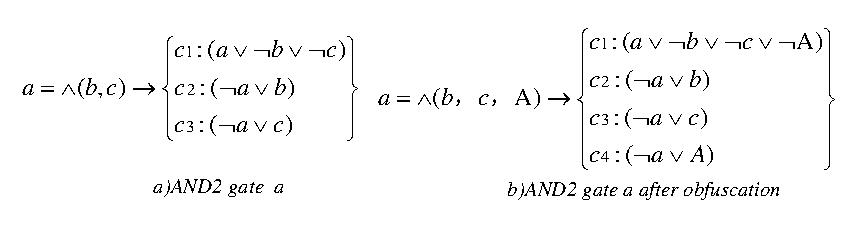
\includegraphics[width=9.2cm]{AND2.eps}}
\caption{将AND2门改变为AND3门.}\centering
%\caption{Obfuscating AND2 into AND3.}\centering
\label{fig_AND2}
\end{figure}

\subsubsection{\textsl{OBFUSCATOR 算法}}

%The proposed OBUFSCATOR algorithm obfuscates CNF formula $F_C$ with SSH rules and CSA strategies,
%so as to prevent structure of $F_C$ and its accurate solution from being known by adversary.
%
%To achieve these goals, OBFUSCATOR detect gates in CNF formula,
%then transform them into gates with different CNF signature.
%Detailed implementation of OBFUSCATOR is in Algorithm \ref{algo_obs}, which use $mark$ $($line \ref{mark}$)$ to detect key clauses and output variables  in CNF formula,
%and use $generate\_new\_clause$ $($line \ref{gennewclause}$)$ to generate new clause.
%As all circuits can be represented by a combination of AND2 and INV,
%and the $mark$ algorithm for INV is trivial,
%so we only present the implementation of $mark$ for AND2 in Algorithm \ref{algo_mark}.
%Similarly, we also present only the implementation of $\mathbf{generate\_new\_clause}$ for AND2 in Algorithm \ref{algo_mark}.
%These two algorithms can transform a CNF signature of AND2 to that of AND3.
OBUFSCATOR算法遵循上述SSH规则和CSA策略,
混淆CNF公式$F_C$,从而防止$F_C$的携带的电路结构和它的真实解被潜在的攻击者获取。

为了达到上述目标,OBFUSCATOR首先会检测CNF公式中的门,
而后将这些门转变为不同标记的门.
OBFUSCATOR的详细实现在算法\ref{algo_obs}中,其中使用$mark$(第$\ref{mark}$行)来检测CNF公式中的关键子句和输出变量,
并使用$generate\_new\_clause$(第$\ref{gennewclause}$行)产生新的子句。
由于AND2是最常见的门,
我们在仅仅给出AND2门的$\mathbf{mark}$算法,
同样,我们也仅仅给出AND2的$\mathbf{generate\_new\_clause}$算法,
这两个算法组合起来可以将AND2的标记转换为AND3的标记.具体的实现在算法\ref{algo_mark}中。

%\begin{algorithm*}[b]
%%\SetAlgoLined
%\SetAlgoNoLine
%\KwData{NULL}
%\KwResult{Husks CNF $F_H$ and Husks result $R_H$}
%\Begin{
%Generating prime numbers $p_A$ and $p_B$  \; \label{primenumber}
%$\Phi= M(I_1 \neq 1, I_2\neq 1, O=p_A*p_B)$ \;\label{multiplePrime}
%$F_H=Tseitin(\Phi)$ \;\label{TseitinPHI}
%$R_H=p_A\mid p_B$ \;
%}
%\caption{GENERATOR}
%\label{algo2_gen}
%\end{algorithm*}

%\begin{algorithm}[t]
%\SetAlgoNoLine
%\KwData{The original CNF $F_C$, Husks CNF $F_H$, Husks result $R_H$}
%\KwResult{The obfuscated CNF $F_O$, variable mapping $M$}
%\Begin{
%$mark(F_C)$\;\label{mark}
%\ForEach{$c\in F_C$}{
%\If{$c \in$  Key Clause Set } {\label{keyclause}
%    lit =get literal $ \in R_H$\;
%    $c=c \cup \neg lit$\;\label{rule1}
%    $nc=generate\_new\_clause(c,lit)$\;\label{gennewclause}
%    $F_C=F_C \cup nc$\;\label{blendclause1}
% }
%}
%\ForEach{$ c \in F_C $} {
%$averagelen=\frac{\sigma _{c'\in F_C}|c'|}{|F_C|}$ \;
%\While{$|c| < averagelen$}{
%$lit=$get literal $\in R_H$ \;
%\While{$\neg lit \in c$} {
%lit=get literal $ \in R_H $ \;
%}
%$c=c \cup \neg lit$\;\label{rule1-2}
%}
%$M$ =remap all variable in $F_C\cup F_H$ \;\label{MV}
%$F_O$ =reorder all clause in $F_C\cup F_H$ \; \label{blendclause2}
%}
%}
%\caption{OBFUSCATOR}
%\label{algo_obs}
%\end{algorithm}
%
%\begin{algorithm}[t]
%\SetAlgoNoLine
%$\mathbf{mark}$\;
%\KwData{CNF formula $S$}
%\KwResult{marked $S$ }
%\Begin{
%\ForEach{$(C \in S) ~\&~ (|C|\equiv 3)$}{
%\ForEach{$l \in C$ }{
%\ForEach{$(C_1 \in S) ~\&~ (\neg l\in C_1)~ \&~ (|C_1|\equiv 2)$ }{
%\ForEach{$l_1 \in C_1$ }{
%\uIf{$(\neg l_1 \in C)~\&~(l_1\ne l)$} {
%$match++$ \;
%}
%}
%}
%}
%}
%\If{$match\equiv 2$} {
%mark $l$ as output literal \;
%mark $C$ as Key Clause\;
%}
%}
%$\mathbf{generate\_new\_clause}$\;
%\KwData{key clause $C$ in AND2, Husk literal $lit$}
%\KwResult{new clause $C_1$}
%\Begin{
%$olit$=Getting output literal from $C$ \;
%$C_1= lit \cup \neg olit$ \;\label{rule2}
%}
%\caption{$\mathbf{mark}$ and $\mathbf{generate\_new\_clause}$}
%\label{algo_mark}
%\end{algorithm}

%SSH and CSA based obfuscation procedure implemented in Algorithm \ref{algo_obs} and \ref{algo_mark} is described below.
%% \textbf{SSO obfuscation with SSH rule and CSA strategy}
%\begin{Procedure}[${Obf_{SSH\_CSA}}$]\label{obsprocedure}~
%\begin{enumerate}
%\item Input:
%Formula $F_C$, Husks formula $F_H$, solution $R_H$.
%\item Output:
%Formula $F_O$.
%\end{enumerate}
%According to Algorithm \ref{algo_obs},
%$F_C$ consists of \textbf{key clause}(line \ref{keyclause}) and \textbf{non-key clause},
%corresponding clause sets denoted as \textbf{$F_{Ck}$} and \textbf{$F_{Cn}$}.
%
%% $~~~~R_H$ is one sultion of $F_H$.
%\textbf{Step 1}:
%For key clause $c\in F_{Ck}$,
%take one literal lit from $R_H$,
%and insert $\neg lit$ into $c$ (at line \ref{rule1}, \ref{rule1-2} in Algorithm \ref{algo_obs})  according to  SSH rule 1.
%% if variable is $T$ in $R_H$, insert its negative literal;
%% if variable is $F$ in $R_H$, insert its positive literal.
%The resulting clause set is denoted as $S_3$ .
%
%\textbf{Step 2}:
%Generating new clauses  (line \ref{gennewclause} in Algorithm \ref{algo_obs}) with literal lit from $R_H$ and output variable of $c$ in $F_C$ according to SSH rule 2 (line \ref{rule2} in Algorithm \ref{algo_mark}).
%% %generating new clauses with literals from $R_H$ and variables in $F_C$ according to the SSH rule 2:
%% if variable is $T$ in $R_H$, insert positive literal into clause;
%% if variable is $F$ in $R_H$, insert negative literal into clause;
%% %Literal of output variable is extracted directly from the key clause and inverted.
%New clauses set generated in this way is denoted as $S_4$.
%
%\textbf{Step 3}:
%Combining and randomly reordering $S_3$, $S_4$, $F_H$, and $F_{Cn}$, to produce $F_O$ (line \ref{rule1}, \ref{rule1-2}, \ref{blendclause1} \ref{blendclause2} in Algorithm \ref{algo_obs}).
%
%\textit{\textbf{end Procedure}}.
%\end{Procedure}

算法\ref{algo_obs}和\ref{algo_mark}中实现的基于SSH和CSA混淆过程描述如下:

\textit{\textbf{Procedure \ref{obsprocedure}}}.
% \textbf{SSO obfuscation with SSH rule and CSA strategy}
%\begin{procedure}[${Obf_{SSH\_CSA}}$]\label{obsprocedure}~
\begin{enumerate}
\item[]\label{obsprocedure} 输入:公式$F_C$, Husks公式$F_H$, 解$R_H$.
\item[] 输出: Formula $F_O$.
\end{enumerate}
根据算法\ref{algo_obs},
$F_C$包含了\textbf{关键子句}(第\ref{keyclause}行)和\textbf{非关键子句},
相应的子句集合表示为\textbf{$F_{Ck}$}和\textbf{$F_{Cn}$}.

% $~~~~R_H$ is one sultion of $F_H$.
\textbf{步骤1}:
对关键子句$c\in F_{Ck}$,
从$R_H$中取出文字$lit$,根据SSH规则1
将$\neg lit$加入到$c$(算法\ref{algo_obs}的\ref{rule1}, \ref{rule1-2}行).
% if variable is $T$ in $R_H$, insert its negative literal;
% if variable is $F$ in $R_H$, insert its positive literal.
生成子句的集合记为$S_3$ .

\textbf{步骤2}:
根据SSH规则2,
使用$R_H$中文字lit和$c$中的输出变量,产生新的子句(算法 \ref{algo_obs}的\ref{gennewclause}行,  算法\ref{algo_mark} 的\ref{rule2}行)。
% %generating new clauses with literals from $R_H$ and variables in $F_C$ according to the SSH rule 2:
% if variable is $T$ in $R_H$, insert positive literal into clause;
% if variable is $F$ in $R_H$, insert negative literal into clause;
% %Literal of output variable is extracted directly from the key clause and inverted.
新产生的子句集合记为$S_4$.

\textbf{步骤3}:
将$S_3$, $S_4$, $F_H$, 和$F_{Cn}$, 混合产生$F_O$ (算法\ref{algo_obs}的\ref{rule1}, \ref{rule1-2}, \ref{blendclause1} \ref{blendclause2} 行).

\textit{\textbf{end Procedure}}.
%\end{procedure}
\subsection{真实解的恢复}\label{mappping}
%After SAT Solving finished in public Cloud, $S_O$,
%the solution of $F_O$, will be returned to the private Cloud.
%In accordance with OBFUSCATOR,
%MAPPER and VERIFIER are used to filter solution of $F_C$ out from  $S_O$.
%MAPPER and VERIFIER are implemented in Algorithm \ref{algo_map}.
%
%According to Theorem \ref{SSOtheorem},
%If result is UNSAT, then the original CNF formula is UNSAT (line \ref{sUNSAT}).
%If result is SAT, MAPPER (line \ref{var}-\ref{mapper}) projects solution into variables of $F_C$ and $F_H$,
%to get $S_C$ and $S_H$, which are the candidate solution of $F_C$ and $F_H$ respectively.
%VERIFIER (line \ref{verifer1}-\ref{verifer2}) checks if $S_H$ is equal to $R_H$,
%if yes, $S_C$ is real solution of  $F_C$.
%Otherwise, $S_C$ may be false solution,
%hence, it is necessary to ask for a new solution from SAT Solver(at line \ref{Warning}).
%
%The solution projection is done according to the variable mapping table $M$,
%generated by OBFUSCATOR(at Line \ref{MV} in Algorithm \ref{algo_obs}).
%$M[var].variable$ (at Line \ref{var}) represents the original variables name of var,
%and $M[var].formula$ (at Line \ref{formula}) may be $F_C$ or $F_H$, which the var belongs to.

在公共云上的求解器完成求解并给出$F_O$解$S_O$,并返回给私有云中。
和混淆器相对应,在私有云中使用MAPPER和VERIFIER将$F_C$的解从$S_O$中过滤出来.
MAPPER和VERIFIER的实现在算法\ref{algo_map}中.

根据定理\ref{SSOtheorem},
如果结果是UNSAT, 那么原始的CNF公式也是(第\ref{sUNSAT}行).
如果结果是SAT, MAPPER(\ref{var}-\ref{mapper}行)将解投影到$F_C$和$F_H$的变量上,
已获得$S_C$ 和$S_H$,分别作为$F_C$和$F_H$的候选解。
VERIFIER (\ref{verifer1}-\ref{verifer2}行)检测$S_H$是否等于$R_H$,
如果等于, $S_C$就是$F_C$的真实解.
否则, $S_C$ 可能是假解,
此时,需要从SAT求解器获得一个新的解(第\ref{Warning}行).

解的投影过程依赖于变量映射表$M$,它由OBFUSCATOR(算法\ref{algo_obs}的\ref{MV}行)创建.
$M[var].variable$ (第\ref{var}行)表示了var的原始变量名,
$M[var].formula$ (第\ref{formula}行)表示var所属于的公式,可以是$F_C$ 或 $F_H$。

\begin{algorithm}[t]
\caption{MAPPER-VERIFIER}
%\SetAlgoNoLine
\begin{algorithmic}[1]
% \SetAlgoNoLine
\STATE input : Obfuscated result $S_O$, variable mapping table $M$, Husk result $R_H$;
\STATE output : Result $S_C$;
\IF{$S_O$ is UNSAT} \label{sUNSAT}
\RETURN UNSAT ;
\ENDIF
\FOR {$lit \in S_O$}
\STATE $var=abs(lit)$;
\STATE $rvar=M[var].variable $;\label{var}
\IF{$M[var].formula ~is~ F_C$}  \label{formula}
\STATE $S_C[rvar]=lit>0?rvar:\neg rvar$ ; \label{mapper}
\ELSE
\STATE $Hlit=lit>0?rvar:\neg rvar$;\label{verifer1}
\IF{$R_H[rvar]\ne Hlit$}
\STATE    alert("Get another Solution from SAT Solver"); \label{Warning}
\STATE    break;
\ENDIF
\ENDIF
\label{verifer2}
\ENDFOR
\PRINT " SAT  solution is $S_C$ ";
\caption{MAPPER and VERIFIER}
\label{algo_map}
\end{algorithmic}
\end{algorithm}

\section{理论分析}
\subsection{正确性证明}\label{correctness}
%According to Theorems \ref{SSEtheorem} and \ref{SSOtheorem}, under SSH rules,
%original CNF formula can be blended with Husks formula seamless, without narrowing down the solution space.
%In this section, we prove these theorems.
%First of all, let's introduce some lemmas.
根据定理\ref{SSOtheorem},在SSH规则下,
原始的CNF公式可以和Husks公式无缝混合, 而不会削减解空间.
本节中,我们证明这些定理。
首先给出以下的引理。

\begin{lemma}[Husks Equation(HE)]\label{HE}

对Husks公式 ${F_H}$且$|V_{F_H}|= n$,
它的全部$m$解$\{S_{H_l}|1\leqslant l\leqslant m\}$,
且解$S_{H_l}=\{y_k=B_{l_k}|B_{l_k} \in \{T,F\}, 1\leqslant k\leqslant n\}$.

对每个$S_{H_l}$, 令$F_{slH}=
(\bigwedge_{1\leqslant i\leqslant n}^{B_{l_i}\equiv T}y_{i})\wedge
(\bigwedge_{1\leqslant j\leqslant n}^{B_{l_j}\equiv F}\neg y_{j})$,

并且令$F_{_SH}=\bigvee_{1\leqslant l\leqslant m}F_{slH}$,

\textbf{则有}  $F_{_SH} \equiv F_H $.
\end{lemma}

\begin{proof}


1) 由于 $F_{_SH} \equiv T$ 则必然存在
% $F_{slH}\equiv T$, for
\begin{equation}
F_{slH}=
(\bigwedge_{1\leqslant i\leqslant n}^{B_{l_i}\equiv T}y_{i})\wedge
(\bigwedge_{1\leqslant j\leqslant n}^{B_{l_j}\equiv F}\neg y_{j}) \equiv T
\end{equation}
则有:
\begin{equation}
S_{H_l}=\{y_{i}=T,y_{j}=F|B_{l_i}\equiv T, B_{l_j}\equiv F, 1\leqslant i, j\leqslant n \}
\end{equation}
令$B_i$, $B_j$分别替换$y_{i}=T$中的$T$和$y_{j}=F$中的$F$, 则有:
\begin{equation}
S_{H_l}=\{(y_i=B_{l_i},y_j=B_{l_j})|B_{l_i}\equiv T, B_{l_j}\equiv F, 1\leqslant i, j\leqslant n\}
\end{equation}
因为$S_{H_l}$是$F_H$的一个解,则有$F_H(S_H/V_{F_H})\equiv T$。则有:
\begin{equation}\label{left}
 F_{_SH} \vdash F_H
\end{equation}
2) 由于 $F_H\equiv T$, 必然存在$F_H$的解,如式(\ref{solution_hl})所示, 可以使$F_H(S_{H_1}/V_{F_H})$ 为真。
\begin{equation}\label{solution_hl}
S_{H_1}=\{y_k=B_{1_k}|B_{1_k} \in \{T,F\}, 1\leqslant k\leqslant n\}.
\end{equation}
根据式(\ref{solution_hl})构造 $F_{s1H}$ ,则有式(\ref{SH}):
\begin{equation}\label{s1H}
F_{s1H}=
(\bigwedge_{1\leqslant i\leqslant n}^{B_{1_i}\equiv T}y_{i})\wedge
(\bigwedge_{1\leqslant j\leqslant n}^{B_{1_j}\equiv F}\neg y_{j})
\end{equation}
\begin{equation}\label{SH}
F_{_SH} =F_ {s1H} \vee (\bigvee_{2\leqslant l\leqslant m}F_{slH}). \\
\end{equation}
因为$F_{s1H} \equiv T$, 并且有式(\ref{s1H})和(\ref{SH}), 则有:
\begin{equation}
F_{_SH}  \equiv T
\end{equation}
\begin{equation}\label{right}
F_H \vdash F_{_SH}
\end{equation}
根据式(\ref{left}) 和 (\ref{right}), 则有:
\begin{equation}
 F_{_SH} \equiv F_H
\end{equation}
%\textit{end proof.}
\end{proof}

%\begin{lemma}[Singular Husk Equation(SHE)]\label{SHE}
%
%对单一Husk公式${F_H}$且有$|V_{F_H}|= n$,
%其唯一解$S_H$=$\{(y_i=B_i,y_j=B_j)|B_i\equiv T, B_j\equiv F, 1\leqslant i, j\leqslant n \}$.
%
%令$F_{_SH}=F_H\wedge (\bigwedge_{1\leqslant i\leqslant n}^{B_i\equiv T}y_i)\wedge(\bigwedge_{1\leqslant j\leqslant n}^{B_j\equiv F}\neg y_j)$
%
%\textbf{则有} $F_H \equiv F_{_SH}$.
%\end{lemma}
%\begin{proof}~\\
%1)因为$F_H\equiv T$, $F_H$有唯一解$S_H$。
% \begin{equation}\label{S_H}
% S_H=\{(y_i=B_i,y_j=B_j)|B_i\equiv T, B_j\equiv F, 1\leqslant i, j\leqslant n \}.
%\end{equation}
%根据式\ref{S_H}),构造$F_{_{lS}H}$
%\begin{equation}
% F_{_{lS}H}=(\bigwedge_{1\leqslant i\leqslant n}^{B_i\equiv T}y_i)\wedge(\bigwedge_{1\leqslant j\leqslant n}^{B_j\equiv F}\neg y_j)
%\end{equation}
%则有
%\begin{equation}
% F_{_{lS}H} \equiv T
%\end{equation}
%构造$F_{_SH}$
%\begin{equation}
% F_{_SH}=F_H\wedge F_{_{lS}H}
%\end{equation}
%则有
%\begin{equation}
% F_{_SH} \equiv T
%\end{equation}
%\begin{equation}
% F_H \vdash F_{_SH}
%\end{equation}\\
%2)因为 $F_{_SH}\equiv T$
%\begin{equation}
%F_{_SH}=(\bigwedge_{1\leqslant i\leqslant n }^{B_i\equiv T}y_i)\wedge(\bigwedge_{1\leqslant j\leqslant n}^{B_j\equiv F}\neg y_j)
%\end{equation}
%则有$F_{_SH}$的唯一解$S_H$
%\begin{equation}
%S_H=\{(y_i=T,y_j=F)|B_i\equiv T, B_j\equiv F, 1\leqslant i, j\leqslant n \}
%\end{equation}
%令 $B_i$替换$T$, $B_j$替换$F$,则有
% \begin{equation}
%S_H=\{(y_i=B_i,y_j=B_j)|B_i\equiv T, B_j\equiv F, 1\leqslant i, j\leqslant n \}
% \end{equation}
%因为$S_H$是$F_H$的解, 则有
%\begin{equation}
%F_H(S_H/V_{F_H})\equiv T
%\end{equation}
% 因此有
% \begin{equation}
%  F_H \vdash F_{_SH}
% \end{equation}
% \\
%因为 1) and 2):
%\begin{equation}
% F_H \equiv F_{_SH}.
%\end{equation}
%\end{proof}

%根据引理\ref{HE}和\ref{SHE},一个单一Husk公式等价于解文字的合取;
%一个Husks公式等价于解子句的析取,其中每个解子句是该解中所有文字的合取。

根据引理\ref{HE},一个Husks公式等价于解子句的析取,其中每个解子句是该解中所有文字的合取。

%%%%%%%%%%%%%%%%%%%%%%%%%%%%%%%%%%%%%%%%%%%%%%%%%%%%%%%%%%%%%%%%%%%%%%%%%%%%%%%%%%%%%%%%%%%%%%%%%%%%%%%%%%%%
%\begin{lemma}[OR Hold Obfuscation]\label{ORrelation-Holding-Obfuscation}
%For formula $F_C$ and $F_{_RH}\vee F_{_SH}$, with $R_H$ is an assignment of $F_{_RH} \vee F_{_SH}$,
%then
%
%$Obf(F_C,F_{_RH}\vee F_{_SH},R_H)\equiv Obf(F_C,F_{_RH},R_H) \vee Obf(F_C,F_{_SH},R_H)$
%\end{lemma}
%\begin{proof}
%Assume
%\begin{enumerate}
% \item[-]$F_C$=$F_{Ck} \wedge F_{Cn}$,  $F_{Ck}$= $\bigwedge_{1}^{m}(a_i\vee X_i$).
% \item[-]$F_H$=$F_{_RH}\vee F_{_SH}$
% \item[-]$R_H$=$\{y_j=B_j| B_j \in \{T,F\}, 1\leqslant j\leqslant n\}$.
% \item[-]Let $F_O=Obf(F_C,F_H,R_H)$
% \end{enumerate}
%% \begin{enumerate}
%% \item[-] Clause $A=a\vee X$,and clause $B=b$, while $b\notin X$,arbitary formula $F_{Cn},F_{_SH}$
%% \item[-] Let $F_{Ck} =A, F_C=F_{Ck} \wedge F_{Cn}$, $F_{_RH}=B$ $F_H=F_{_RH}\vee F_{_SH}$, while $R_H=\{b\equiv T\}$;
%% \item[-] Let $F_O=Obf(F_C,F_H,R_H)$
%% \end{enumerate}
%%  ~~~~then $F_O=(F_C\wedge F_H) \vee Obf(F_C,F_{_SH} ,R_H$
%According to \textbf{Procedure} \ref{obsprocedure}, construct $F_O$ as following 3 \textbf{steps}.
%\begin{enumerate}
%\item With $(y_j\equiv B_j)\in$ $R_H$, $(a_i\vee X_i) \in F_{Ck}$ and Rule 1:
%\begin{itemize}
% \item[] if $B_j\equiv T$, then clause $C_{ij}=(a_i\vee X_i)\wedge \neg y_j$.
% \item[] if $B_j\equiv F$, then clause $C_{ij}=(a_i\vee X_i)\wedge y_j$.
%\end{itemize}
%and $S_3=\bigwedge_{1\leqslant i\leqslant m}^{1\leqslant j\leqslant n} C_{ij}$
%\item
%With $(y_j\equiv  B_j)\in $ $R_H$, $(a_i\vee X_i) \in F_{Ck}$ and Rule 2:
%\begin{itemize}
% \item[] if $B_j\equiv T$, then clause $D_{ij}=\neg a_i\wedge y_j$.
% \item[] if $B_j\equiv F$, then clause $D_{ij}=\neg a_i\wedge \neg y_j$.
%\end{itemize}
%and $S_4=\bigwedge_{1\leqslant i\leqslant m}^{1\leqslant j\leqslant n} D_{ij}$.
%\item\label{ORFO}
%Let  $F_{_dC} =S_3\wedge S_4 \wedge F_{Cn}$, then $F_O=F_H \wedge F_{_dC}$.
%\end{enumerate}
%According to Step \ref{ORFO}):
%\begin{equation}\label{FOOBF}
%\begin{array}{ccc}
%F_O  =  F_H \wedge F_{_dC}                                   &F_H=F_{_RH}\vee F_{_SH}&\models\\
%F_O  =  (F_{_RH}\vee F_{_SH})\wedge F_{_dC}                  &                       &\models\\
%F_O  =  (F_{_RH} \wedge F_{_dC})\vee(F_{_SH}\wedge F_{_dC})  &                       &
%\end{array}
%\end{equation}
%According to \textbf{Procedure} \ref{obsprocedure}, $F_{_dC}$ is only relevent to $F_C$ and $R_H$, then \\
%% \begin{equation}
%%  Obf(F_C,F_H,R_H) \equiv F_H \wedge F_{_dC}
%% \end{equation}
%\begin{equation}\label{SHOBF}
%F_{_SH} \wedge F_{_dC} \equiv Obf(F_C,F_{_SH},R_H)
%\end{equation}
%\begin{equation}\label{RHOBF}
%F_{_RH} \wedge F_{_dC} \equiv Obf(F_C,F_{_RH},R_H)
%\end{equation}
%According to Equation (\ref{FOOBF}), (\ref{SHOBF}), (\ref{RHOBF}), we have:
% \begin{equation}
%F_O \equiv Obf(F_C,F_{_RH} ,R_H)
%\vee Obf(F_C,F_{_SH} ,R_H)
% \end{equation}
%
%%\textit{end proof.}
%\end{proof}
%
%% \begin{lemma}[AND Hold Obfuscation]\label{ANDrelation-Holding-Obfuscation}
%\begin{lemma}[AND Hold Obfuscation]\label{ANDrelation-Holding-Obfuscation}
%For formula $F_C$ and $F_{_RH}\wedge F_{_SH}$,
%with $R_H$ is an assignment of $F_{_RH} \wedge F_{_SH}$, then
%
%$Obf(F_C,F_{_RH} \wedge F_{_SH},R_H) $ \\
%$\equiv Obf(F_C,F_{_RH},R_H) \wedge Obf(F_C,F_{_SH} ,R_H)$
%\end{lemma}
%\begin{proof}
%\textsl{Abbr.}
%Similar to Lemma \ref{ORrelation-Holding-Obfuscation}.
%% \textbf{Assume}
%% \begin{enumerate}
%% \item[-] Clause $A=a\vee X$,and clause $B=b$, while $b\notin X$,arbitary formula $F_{Cn},F_{_SH}$
%% \item[-] Let $F_{Ck} =A, F_C=F_{Ck} \wedge F_{Cn}$, \\
%%           $F_{_RH}=B, F_H=F_{_RH}\wedge F_{_SH}$, while $R_H=\{b\equiv T\}$;
%% \item[-] Let $F_O=Obf(F_C,F_H,R_H)$
%% \end{enumerate}
%% % then $F_O=Obf(F_C,F_{_RH},R_H)\wedge Obf(F_C,F_{_SH},R_H)$.
%% According to \textbf{Procedure} \ref{obsprocedure}, construct $F_O$ as following 3 steps.
%% \begin{enumerate}
%% \item With $R_H$ and Rule 1,
%% we have clause $C=A\vee \neg b$, and $S_3=C$
%% \item
%% With $R_H$ and Rule 2,
%% with literal $a\in A$,
%% we have clause $D=\neg a\vee b$;
%% and $S_4=D$;
%% \item
%% Let  $F_{_dC} =S_3\wedge S_4 \wedge F_{Cn}$.\\
%% then $F_O=F_H \wedge F_{_dC}$.
%% \end{enumerate}
%% \begin{equation}
%% \begin{array}{ccc}
%% F_O  =  F_H \wedge F_{_dC}                                     & F_H=F_{_RH}\wedge F_{_SH}&\models\\
%% F_O  =  (F_{_RH}\wedge F_{_SH})\wedge F_{_dC}                   &                        &\models\\
%% F_O  =  (F_{_RH} \wedge F_{_dC})\wedge (F_{_SH} \wedge F_{_dC})  &                        &\models\\
%% \end{array}
%% \end{equation}
%% According to \textbf{Procedure} \ref{obsprocedure}, $F_{_dC}$ is only relevent to $F_C$ and $R_H$, then\\
%% $F_{_SH} \wedge F_{_dC} \equiv Obf(F_C,F_{_SH},R_H)$\\
%% $F_{_RH} \wedge F_{_dC} \equiv Obf(F_C,F_{_RH},R_H)$
%%
%% $F_O  = Obf(F_C,F_{_RH},R_H)\wedge Obf(F_C,F_{_SH},R_H)$
%%
%% \textit{end proof.}
%\end{proof}
%
%According to Lemma \ref{ORrelation-Holding-Obfuscation} and \ref{ANDrelation-Holding-Obfuscation},
%for Husk formula $F_H$,  AND and OR relation are true after obfuscation.


\begin{lemma}[OR Hold Obfuscation]\label{ORrelation-Holding-Obfuscation}
对公式$F_C$ 和$F_{_RH}\vee F_{_SH}$,及$F_{_RH} \vee F_{_SH}$的一个赋值$R_H$ 有,

$Obf(F_C,F_{_RH}\vee F_{_SH},R_H)\equiv Obf(F_C,F_{_RH},R_H) \vee Obf(F_C,F_{_SH},R_H)$
\end{lemma}
\begin{proof}
假设:
\begin{enumerate}
 \item[-]$F_C$=$F_{Ck} \wedge F_{Cn}$,  $F_{Ck}$= $\bigwedge_{1}^{m}(a_i\vee X_i$).
 \item[-]$F_H$=$F_{_RH}\vee F_{_SH}$
 \item[-]$R_H$=$\{y_j=B_j| B_j \in \{T,F\}, 1\leqslant j\leqslant n\}$.
 \item[-]令 $F_O=Obf(F_C,F_H,R_H)$
 \end{enumerate}
% \begin{enumerate}
% \item[-] Clause $A=a\vee X$,and clause $B=b$, while $b\notin X$,arbitary formula $F_{Cn},F_{_SH}$
% \item[-] Let $F_{Ck} =A, F_C=F_{Ck} \wedge F_{Cn}$, $F_{_RH}=B$ $F_H=F_{_RH}\vee F_{_SH}$, while $R_H=\{b\equiv T\}$;
% \item[-] Let $F_O=Obf(F_C,F_H,R_H)$
% \end{enumerate}
%  ~~~~then $F_O=(F_C\wedge F_H) \vee Obf(F_C,F_{_SH} ,R_H$
根据\textbf{Procedure}\ref{obsprocedure},按下列3个\textbf{步骤}构造$F_O$.
\begin{enumerate}
\item  $(y_j\equiv B_j)\in$ $R_H$, $(a_i\vee X_i) \in F_{Ck}$和规则1:
\begin{itemize}
 \item[] 如果$B_j\equiv T$, 则子句$C_{ij}=(a_i\vee X_i)\wedge \neg y_j$.
 \item[] 如果$B_j\equiv F$, 则子句$C_{ij}=(a_i\vee X_i)\wedge y_j$.
\end{itemize}
令$S_3=\bigwedge_{1\leqslant i\leqslant m}^{1\leqslant j\leqslant n} C_{ij}$
\item
$(y_j\equiv  B_j)\in $ $R_H$, $(a_i\vee X_i) \in F_{Ck}$以及规则2:
\begin{itemize}
 \item[] 如果$B_j\equiv T$, 则子句$D_{ij}=\neg a_i\wedge y_j$.
 \item[] 如果$B_j\equiv F$, 则子句$D_{ij}=\neg a_i\wedge \neg y_j$.
\end{itemize}
令$S_4=\bigwedge_{1\leqslant i\leqslant m}^{1\leqslant j\leqslant n} D_{ij}$.
\item\label{ORFO}
令$F_{_dC} =S_3\wedge S_4 \wedge F_{Cn}$, then $F_O=F_H \wedge F_{_dC}$.
\end{enumerate}
根据步骤\ref{ORFO}):
\begin{equation}\label{FOOBF}
\begin{array}{ccc}
F_O  =  F_H \wedge F_{_dC}                                   &F_H=F_{_RH}\vee F_{_SH}&\models\\
F_O  =  (F_{_RH}\vee F_{_SH})\wedge F_{_dC}                  &                       &\models\\
F_O  =  (F_{_RH} \wedge F_{_dC})\vee(F_{_SH}\wedge F_{_dC})  &                       &
\end{array}
\end{equation}
根据\textbf{Procedure}\ref{obsprocedure}, $F_{_dC}$仅和$F_C$以及$R_H$相关, 则\\
% \begin{equation}
%  Obf(F_C,F_H,R_H) \equiv F_H \wedge F_{_dC}
% \end{equation}
\begin{equation}\label{SHOBF}
F_{_SH} \wedge F_{_dC} \equiv Obf(F_C,F_{_SH},R_H)
\end{equation}
\begin{equation}\label{RHOBF}
F_{_RH} \wedge F_{_dC} \equiv Obf(F_C,F_{_RH},R_H)
\end{equation}
根据式(\ref{FOOBF}), (\ref{SHOBF}), (\ref{RHOBF}), 有:
 \begin{equation}
F_O \equiv Obf(F_C,F_{_RH} ,R_H)
\vee Obf(F_C,F_{_SH} ,R_H)
 \end{equation}

%\textit{end proof.}
\end{proof}

% \begin{lemma}[AND Hold Obfuscation]\label{ANDrelation-Holding-Obfuscation}
\begin{lemma}[AND Hold Obfuscation]\label{ANDrelation-Holding-Obfuscation}
公式$F_C$ 和$F_{_RH}\wedge F_{_SH}$,
并且$R_H$是$F_{_RH} \wedge F_{_SH}$的一个赋值, 则有

$Obf(F_C,F_{_RH} \wedge F_{_SH},R_H) $ \\
$\equiv Obf(F_C,F_{_RH},R_H) \wedge Obf(F_C,F_{_SH} ,R_H)$
\end{lemma}
\begin{proof}
%\textsl{略.}
%同Lemma \ref{ORrelation-Holding-Obfuscation}.
 \textbf{假设}
 \begin{enumerate}
 \item[-] 子句 $A=a\vee X$ 和 $B=b$, 并且 $b\notin X$, 任意公式 $F_{Cn},F_{_SH}$
 \item[-] 令 $F_{Ck} =A, F_C=F_{Ck} \wedge F_{Cn}$, \\
           $F_{_RH}=B, F_H=F_{_RH}\wedge F_{_SH}$, 当$R_H=\{b\equiv T\}$;
 \item[-] 令 $F_O=Obf(F_C,F_H,R_H)$
 \end{enumerate}
 % then $F_O=Obf(F_C,F_{_RH},R_H)\wedge Obf(F_C,F_{_SH},R_H)$.
 根据\textbf{Procedure} \ref{obsprocedure}, 按下列3个步骤构造$F_O$。
 \begin{enumerate}
 \item 根据$R_H$和规则1,
 构造子句 $C=A\vee \neg b$, 令子句集合 $S_3=C$
 \item
 根据 $R_H$ 和规则 2,
 对于文字 $a\in A$,
 构造子句 $D=\neg a\vee b$;
 令子句集合 $S_4=D$;
 \item
 令 $F_{_dC} =S_3\wedge S_4 \wedge F_{Cn}$.\\
 则有 $F_O=F_H \wedge F_{_dC}$.
 \end{enumerate}
 \begin{equation}\label{ANDequation}
 \begin{array}{ccc}
 F_O  =  F_H \wedge F_{_dC}                                     & F_H=F_{_RH}\wedge F_{_SH}&\models\\
 F_O  =  (F_{_RH}\wedge F_{_SH})\wedge F_{_dC}                   &                        &\models\\
 F_O  =  (F_{_RH} \wedge F_{_dC})\wedge (F_{_SH} \wedge F_{_dC})  &                        &\models\\
 \end{array}
 \end{equation}
 根据\textbf{Procedure} \ref{obsprocedure}, $F_{_dC}$仅仅和$F_C$、$R_H$相关, 则
\begin{equation}\label{FSHequation}
 F_{_SH} \wedge F_{_dC} \equiv Obf(F_C,F_{_SH},R_H)
\end{equation}
\begin{equation}\label{FRHequation}
 F_{_RH} \wedge F_{_dC} \equiv Obf(F_C,F_{_RH},R_H)
\end{equation}
根据式\ref{ANDequation})、\ref{FSHequation})和\ref{FRHequation}),则有
\begin{equation}
 F_O  = Obf(F_C,F_{_RH},R_H)\wedge Obf(F_C,F_{_SH},R_H)
\end{equation}
%\
%textit{end proof.}
\end{proof}

根据引理\ref{ORrelation-Holding-Obfuscation}和\ref{ANDrelation-Holding-Obfuscation},
对Husks公式$F_H$, 公式的与和非关系在混淆后依然保持。
%%%%%%%%%%%%%%%%%%%%%%%%%%%%%%%%%%%%%%%%%%%%%%%%%%%%%%%%%%%%%%%%%%%%%%%%%%%%%%%%%%%%%%%%%%%%%%%%%%%%%%%%%%%%%%%%%%%%%%%%%%%%%%%
%\begin{lemma}[Unique Positive literal SSE Obfuscation]\label{UPSSE-lemma}
%% \textbf{(Unique Positive literal SSE Obfuscation)}
%For any CNF formula $F_C$, we have
%
%\textbf{$Obf(F_C,B=b,{b\equiv T})\equiv F_C\wedge b$}
%\end{lemma}
%\begin{proof}
%%\textbf{Unique Positive literal SSE Obfuscation (UPSSE)}:\label{UPSSE-lemma}
%Assume
%\begin{enumerate}
% \item[-]$F_C$=$F_{Ck} \wedge F_{Cn}$, $F_{Ck}=A$, $A=a\vee X$.
% \item[-]$F_H$=$B$, $B=b$~while $b\notin X$, $R_H$=$\{b\equiv T\}$.
% \item[-]Let $F_O=Obf(F_C,F_H,R_H)$
% \end{enumerate}
%% \begin{enumerate}
%% \item[-] Clause $A=a\vee X$, an arbitary formula $F_{Cn}$ and clause $B=b$, while $b\notin X$;
%% \item[-] Let $F_{Ck} =A, F_C=F_{Ck} \wedge F_{Cn}$, $F_H=B$, while $R_H=\{b\equiv T\}$;
%% \item[-] Let $F_O=Obf(F_C,F_H,R_H)$
%% \end{enumerate}
%%  ~~~~then $F_O=F_C\wedge F_H$.
%According to \textbf{Procedure} \ref{obsprocedure}, Construct $F_O$ as following 3 \textbf{steps}.
%\begin{enumerate}
%\item With $(b\equiv T) \in $ $R_H$ and Rule 1,
%we have clause $C=A\vee \neg b$, and $S_3=C$.
%\item
%With ($b\equiv T) \in $ $R_H$, literal $a\in A$ and Rule 2,
%we have clause $D=\neg a\vee b$,
%and $S_4=D$.
%\item \label{UPSSEFO}
%let $F_O=F_H \wedge S_3\wedge S_4 \wedge F_{Cn}$.
%\end{enumerate}
%According to Step \ref{UPSSEFO}):
%\begin{equation}
%\begin{array}{ccc}
%F_O  =  F_H \wedge S_3\wedge S_4\wedge F_{Cn}           &S_3=C~ S_4=D              &\models\\
%F_O  =  F_H\wedge C\wedge D\wedge F_{Cn}                &F_H=B~ B=b                &\models\\
%F_O  =  b\wedge C\wedge D\wedge F_{Cn}                  &C=A\vee \neg b~           &\models\\
%F_O  =  b\wedge (A\vee \neg b) \wedge D\wedge F_{Cn}    &                          &\models\\
%F_O  =  b\wedge A \wedge D\wedge F_{Cn}                 & D=\neg a\vee b~          &\models\\
%F_O  =  b\wedge A \wedge (\neg a\vee b)\wedge F_{Cn}    &                          &\models\\
%F_O  =  b\wedge A \wedge F_{Cn}                         &F_{Ck} =A                 &\models\\
%F_O  =  b\wedge F_{Ck}\wedge F_{Cn}                     & F_C=F_{Ck} \wedge F_{Cn} &\models\\
%F_O  =  F_C \wedge b                                    &   &
%\end{array}
%\end{equation}
%%\textit{end proof.}
%\end{proof}
%
%\begin{lemma}[Unique Negative literal SSE Obfuscation]\label{UNSSE-lemma}
%For any CNF formula $F_C$, we have
%
% \textbf{$Obf(F_C,B=\neg b,{b=F})=F_C\wedge \neg b$}
%% % Lemma \ref{UNSSE-lemma} can be expressed as following:
%\end{lemma}
%\begin{proof}
% \textsl{Abbr.}
%  Similar to Lemma \ref{UPSSE-lemma}.
%\end{proof}
%% \begin{proof}
%%
%% \begin{enumerate}
%% \item Clause $A=a\vee X$, arbitary formula $F_{Cn}$ and clause $B=\neg b$, while $b\notin X$;
%% \item Let $F_{Ck} =A, F_C=F_{Ck} \wedge F_{Cn}$, $F_H=B$, while $R_H=\{b\equiv F\}$;
%% \item Let $F_O=Obf(F_C,F_H,R_H)$
%% \end{enumerate}
%%  ~~~~then $F_O=F_C\wedge F_H$.
%
%% According to \textbf{Procedure} \ref{obsprocedure}, Construct $F_O$ as following 3 steps.
%% \begin{enumerate}
%% \item[Step1]
%% With $R_H$ and Rule 1,
%% we have clause $C=A\vee b$;and $S_3=C$
%% \item[Step2]
%% With $R_H$ and Rule 2,
%% with literal $a\in A$,
%% we have clause $D=\neg a\vee \neg b$;
%% and $S_4=D$;
%% \item[Step3] let $F_O=F_H \wedge S_3\wedge S_4 \wedge F_{Cn} $.
%% \end{enumerate}
%% \begin{equation}
%% \begin{array}{ccc}
%% F_O  =  F_H \wedge S_3\wedge S_4\wedge F_{Cn}                      &F_H=B      &\models\\
%% F_O  =  B \wedge S_3\wedge S_4\wedge F_{Cn}                        &S_3=C      &\models\\
%% F_O  =  B \wedge C\wedge S_4\wedge F_{Cn}                          &S_4=D      &\models\\
%% F_O  =  B\wedge C\wedge D\wedge F_{Cn}                             &B=\neg b                    &\models\\
%% F_O  =  \neg b\wedge C\wedge D\wedge F_{Cn}                        &C=A\vee b               &\models\\
%% F_O  =  \neg b\wedge (A\vee  b) \wedge D\wedge F_{Cn}              &                            &\models\\
%% F_O  =  \neg b\wedge A \wedge D\wedge F_{Cn}                       &D=\neg a\vee \neg b     &\models\\
%% F_O  =  \neg b\wedge A \wedge (\neg a\vee \neg b)\wedge F_{Cn}     &                            &\models\\
%% F_O  =  \neg b\wedge A \wedge F_{Cn}                               &F_{Ck}=A                    &\models\\
%% F_O  =  \neg b\wedge F_{Ck}\wedge F_{Cn}                        & F_C=F_{Ck} \wedge F_{Cn}   &\models\\
%% F_O  =  F_C\wedge \neg b                                           &   &
%% \end{array}
%% \end{equation}
%%
%% \textit{end proof.}
%% \end{proof}
%
%According to Lemma \ref{UPSSE-lemma} and \ref{UNSSE-lemma},
%after unique literal obfuscation, solution space is unchanged.

%\begin{lemma}[Unique Positive literal SSE Obfuscation]\label{UPSSE-lemma}
%% \textbf{(Unique Positive literal SSE Obfuscation)}
%任意公式$F_C$, 有
%
%\textbf{$Obf(F_C,B=b,{b\equiv T})\equiv F_C\wedge b$}
%\end{lemma}
%\begin{proof}
%%\textbf{Unique Positive literal SSE Obfuscation (UPSSE)}:\label{UPSSE-lemma}
%假设
%\begin{enumerate}
% \item[-]$F_C$=$F_{Ck} \wedge F_{Cn}$, $F_{Ck}=A$, $A=a\vee X$.
% \item[-]$F_H$=$B$, $B=b$~while $b\notin X$, $R_H$=$\{b\equiv T\}$.
% \item[-]Let $F_O=Obf(F_C,F_H,R_H)$
% \end{enumerate}
%% \begin{enumerate}
%% \item[-] Clause $A=a\vee X$, an arbitary formula $F_{Cn}$ and clause $B=b$, while $b\notin X$;
%% \item[-] Let $F_{Ck} =A, F_C=F_{Ck} \wedge F_{Cn}$, $F_H=B$, while $R_H=\{b\equiv T\}$;
%% \item[-] Let $F_O=Obf(F_C,F_H,R_H)$
%% \end{enumerate}
%%  ~~~~then $F_O=F_C\wedge F_H$.
%根据\textbf{Procedure} \ref{obsprocedure}, 按下列3个步骤构造$F_O$。
%\begin{enumerate}
%\item $(b\equiv T) \in $ $R_H$以及规则1,
%有子句$C=A\vee \neg b$, 并且 $S_3=C$.
%\item
%($b\equiv T) \in $ $R_H$, literal $a\in A$和规则2,
%有子句$D=\neg a\vee b$,
%令$S_4=D$.
%\item \label{UPSSEFO}
%令$F_O=F_H \wedge S_3\wedge S_4 \wedge F_{Cn}$.
%\end{enumerate}
%根据步骤\ref{UPSSEFO}):
%\begin{equation}
%\begin{array}{ccc}
%F_O  =  F_H \wedge S_3\wedge S_4\wedge F_{Cn}           &S_3=C~ S_4=D              &\models\\
%F_O  =  F_H\wedge C\wedge D\wedge F_{Cn}                &F_H=B~ B=b                &\models\\
%F_O  =  b\wedge C\wedge D\wedge F_{Cn}                  &C=A\vee \neg b~           &\models\\
%F_O  =  b\wedge (A\vee \neg b) \wedge D\wedge F_{Cn}    &                          &\models\\
%F_O  =  b\wedge A \wedge D\wedge F_{Cn}                 & D=\neg a\vee b~          &\models\\
%F_O  =  b\wedge A \wedge (\neg a\vee b)\wedge F_{Cn}    &                          &\models\\
%F_O  =  b\wedge A \wedge F_{Cn}                         &F_{Ck} =A                 &\models\\
%F_O  =  b\wedge F_{Ck}\wedge F_{Cn}                     & F_C=F_{Ck} \wedge F_{Cn} &\models\\
%F_O  =  F_C \wedge b                                    &   &
%\end{array}
%\end{equation}
%%\textit{end proof.}
%\end{proof}
%
%\begin{lemma}[Unique Negative literal SSE Obfuscation]\label{UNSSE-lemma}
%任意公式$F_C$, 有
%
% \textbf{$Obf(F_C,B=\neg b,{b=F})=F_C\wedge \neg b$}
%% % Lemma \ref{UNSSE-lemma} can be expressed as following:
%\end{lemma}
%%\begin{proof}
%% \textsl{略.}
%%  同Lemma\ref{UPSSE-lemma}.
%%\end{proof}
% \begin{proof}
%
% \begin{enumerate}
% \item Clause $A=a\vee X$, arbitary formula $F_{Cn}$ and clause $B=\neg b$, while $b\notin X$;
% \item Let $F_{Ck} =A, F_C=F_{Ck} \wedge F_{Cn}$, $F_H=B$, while $R_H=\{b\equiv F\}$;
% \item Let $F_O=Obf(F_C,F_H,R_H)$
% \end{enumerate}
%  ~~~~then $F_O=F_C\wedge F_H$.
%
% According to \textbf{Procedure} \ref{obsprocedure}, Construct $F_O$ as following 3 steps.
% \begin{enumerate}
% \item[Step1]
% With $R_H$ and Rule 1,
% we have clause $C=A\vee b$;and $S_3=C$
% \item[Step2]
% With $R_H$ and Rule 2,
% with literal $a\in A$,
% we have clause $D=\neg a\vee \neg b$;
% and $S_4=D$;
% \item[Step3] let $F_O=F_H \wedge S_3\wedge S_4 \wedge F_{Cn} $.
% \end{enumerate}
% \begin{equation}
% \begin{array}{ccc}
% F_O  =  F_H \wedge S_3\wedge S_4\wedge F_{Cn}                      &F_H=B      &\models\\
% F_O  =  B \wedge S_3\wedge S_4\wedge F_{Cn}                        &S_3=C      &\models\\
% F_O  =  B \wedge C\wedge S_4\wedge F_{Cn}                          &S_4=D      &\models\\
% F_O  =  B\wedge C\wedge D\wedge F_{Cn}                             &B=\neg b                    &\models\\
% F_O  =  \neg b\wedge C\wedge D\wedge F_{Cn}                        &C=A\vee b               &\models\\
% F_O  =  \neg b\wedge (A\vee  b) \wedge D\wedge F_{Cn}              &                            &\models\\
% F_O  =  \neg b\wedge A \wedge D\wedge F_{Cn}                       &D=\neg a\vee \neg b     &\models\\
% F_O  =  \neg b\wedge A \wedge (\neg a\vee \neg b)\wedge F_{Cn}     &                            &\models\\
% F_O  =  \neg b\wedge A \wedge F_{Cn}                               &F_{Ck}=A                    &\models\\
% F_O  =  \neg b\wedge F_{Ck}\wedge F_{Cn}                        & F_C=F_{Ck} \wedge F_{Cn}   &\models\\
% F_O  =  F_C\wedge \neg b                                           &   &
% \end{array}
% \end{equation}
%
% \textit{end proof.}
% \end{proof}
%
%根据Lemma \ref{UPSSE-lemma}和\ref{UNSSE-lemma},
%单文字混淆后解空间保持等价。
%%%%%%%%%%%%%%%%%%%%%%%%%%%%%%%%%%%%%%%%%%%%%%%%%%%%%%%%%%%%%%%%%%%%%%%%%%%%%%%%%%%%%%%%%%%%%%%%%%%%%%%%%%%%%%%%%%%%%%

%Then let's discuss SSE Obfuscation based on singular Husk formula,
%and SSO Obfuscation based on Husks formula.
%
%\textbf{Theorem \ref{SSEtheorem} Solution Space Equated (SSE) Obfuscation}
%
%For arbitrary CNF formula $F_C$, and Singular Husk formula $F_{_SH}$, if
%\begin{enumerate}
% \item[-] $V_{F_C}$ $\cap$ $V_{F_H}$ = $\phi$, $R_H$ is unique solutions of $F_H$.
% \item[-] $F_O=Obf(F_C,F_H,R_H)$.
%\end{enumerate}
%~~~then  $F_C\wedge F_H \equiv F_O$.
%\begin{proof}
%
%Assume $R_H$=$\{y_k=B_k| B_k \in \{T,F\}, 1\leqslant k\leqslant n\}$.
%
%According to \textbf{Procedure} \ref{obsprocedure}, constuct $F_O$ as following \textbf{steps}:
%\begin{enumerate}
%\item \label{Fop}
%Let $F_{Op}=F_C$.  \\
%% for all $B_i\equiv T$, let
%for $y_i \in \{y_i|(y_i=B_{i})\in R_H \parallel B_i\equiv T)\}$, let
%\begin{itemize}
% \item[] $F_{Op}$=$Obf(F_{Op},B=y_i,{y_i\equiv B_i})$.
%\end{itemize}
%\item  \label{Fonp}
%Let $F_{On}=F_{Op}$. \\
%% for all $B_j\equiv F$, let
%for $y_j \in \{y_j|(y_j=B_j)\in R_H \parallel B_j\equiv F)\}$, let
%\begin{itemize}
% \item[] $F_{On}$= $Obf(F_{On},B=\neg y_j,{y_j\equiv B_j})$.
%\end{itemize}
%\item  \label{SSEFOend}
%$F_{O}=F_{On}\wedge F_H$.
%\end{enumerate}
%According to Lemma \ref{ANDrelation-Holding-Obfuscation}, \ref{UPSSE-lemma} and Step \ref{Fop}), we have:
%\begin{equation}\label{SSEFOP}
%F_{Op} \equiv F_C\wedge (\bigwedge_{1\leqslant i\leqslant n}^{B_i \equiv T}y_i)
%\end{equation}
%According to Lemma \ref{ANDrelation-Holding-Obfuscation}, \ref{UNSSE-lemma} and Step \ref{Fonp}), we have:
%\begin{equation}\label{SSEFON}
%F_{On} \equiv F_{Op}\wedge (\bigwedge_{1\leqslant j\leqslant n}^{B_j \equiv F}\neg y_j).
%\end{equation}
%% then
%% \begin{equation}\label{SSEOPN}
%% F_{On} \equiv F_C \wedge
%% (\bigwedge_{1\leqslant i\leqslant n}^{B_i \equiv T}y_i)\wedge
%% (\bigwedge_{1\leqslant j\leqslant n}^{B_j \equiv F}\neg y_j)\\
%% \end{equation}
%According to Step \ref{SSEFOend}) and Equation (\ref{SSEFOP}) (\ref{SSEFON}), we have:
%\begin{equation}\label{SSEFO}
%F_{O} \equiv F_C \wedge
%(\bigwedge_{1\leqslant i\leqslant n}^{B_i \equiv T}y_i)\wedge
%(\bigwedge_{1\leqslant j\leqslant n}^{B_j \equiv F}\neg y_j) \wedge F_H
%\end{equation}
%Since ${R_H}$ is the unique satisfied solution of $F_H$,
%according to Lemma \ref{SHE}, we have:
%\begin{equation}\label{SSEFH}
%F_H \wedge (\bigwedge_{1\leqslant i\leqslant n}^{B_i \equiv T}y_i)\wedge
%(\bigwedge_{1\leqslant j\leqslant n}^{B_j\equiv F}\neg y_j)\equiv F_H
%\end{equation}
%According to Equation (\ref{SSEFO}), (\ref{SSEFH}), we have:
%\begin{equation}\label{SSEEND}
%F_O\equiv F_C \wedge F_H
%\end{equation}
%Since $F_H$ is satisfiable, $V_{F_C}$ $\cap$ $V_{F_H}$ = $\phi$, we have Inference:
%\begin{equation}
%F_O\equiv_{_{SSE}}  F_C
%\end{equation}
%%\textit{end proof.}
%\end{proof}
%
%\textbf{Theorem \ref{SSOtheorem} Solution Space Overapproximated (SSO) Obfuscation}
%
%For arbitrary CNF formula $F_C$, Husks formula $F_H$, if
%\begin{enumerate}
% \item $V_{F_C}$ $\cap$ $V_{F_H}$ = $\phi$, $R_H$ is one of $m$ solutions of $F_H$.
% \item $F_O=Obf(F_C,F_H,R_H)$.
%\end{enumerate}
%~~~Then $F_C \vdash_{_{SSO}} F_O$.
%%\end{theorem}
%\begin{proof}
%
%Assume
%        one solution of $F_H$ is $R_H$=$\{y_i=B_{R_k}|B_{R_k} \in \{T,F\}, 1\leqslant k\leqslant n\}$,
%        and its all other $m-1$ solutions $\{S_{H_l} | 1\leqslant l\leqslant m-1\}$.
%        $S_{H_l}=\{y_k=B_{l_k}|B_{l_k}\in \{ T,F \},~1\leqslant k\leqslant n\}$.
%
%        According to $R_H$ and $S_H$, let's define $F_{_RH}$ and $F_{_SH}$:
%        \begin{equation}\label{SSORH}
%        F_{_RH}=
%        (\bigwedge_{1\leqslant i\leqslant n}^{B_{R_i}\equiv T}y_i)\wedge
%        (\bigwedge_{1\leqslant j\leqslant n}^{B_{R_j}\equiv F}\neg y_j)
%        \end{equation}
%        \begin{equation}\label{SSOSH}
%         F_{_SH}=\bigvee_{1\leqslant l\leqslant m-1}(
%        (\bigwedge_{1\leqslant i\leqslant n}^{B_{l_i}\equiv T}y_i)\wedge
%        (\bigwedge_{1\leqslant j\leqslant n}^{B_{l_j}\equiv F}\neg y_j))   \\
%	  \end{equation}
%According to Lemma \ref{HE}, we have:\\
%        \begin{equation}\label{SSOEquation}
%        F_{_RH}\vee F_{_SH}\equiv F_H
%        \end{equation}
%With $F_O=Obf(F_C,F_H,R_H)$ and Equation (\ref{SSOEquation}), we have:\\
%        \begin{equation}\label{SSOE2}
%	F_O \equiv Obf(F_C,F_{_RH}\vee F_{_SH},R_H)
%        \end{equation}
%According to Lemma \ref{ORrelation-Holding-Obfuscation} and Equation (\ref{SSOE2}), we have:\\
%        \begin{equation}\label{SSOE3}
%	  F_O=Obf(F_C,F_{_RH},R_H) \vee Obf(F_C,F_{_SH},R_H)
%	\end{equation}
%According to Theorem \ref{SSEtheorem}, we have:\\
%	\begin{equation}\label{SSOE4}
%	  Obf(F_C,F_{_RH},R_H)\equiv F_C\wedge F_{_RH}
%        \end{equation}
%With Equation (\ref{SSOE3}) and (\ref{SSOE4}), we have:\\
%        \begin{equation}\label{SSOE5}
%	  F_O \equiv (F_C\wedge F_{_RH}) \vee Obf(F_C,F_{_SH},R_H)
%	\end{equation}
%With Equation (\ref{SSOE5}), we have:\\
%	 \begin{equation}\label{SSOE6}
%	  F_C \wedge F_{_RH}\vdash_{_{SSO}} F_{O} \\
%	\end{equation}
%Since $F_{_RH}$ is satisfiable, $V_{F_C}$ $\cap$ $V_{F_H}$ = $\phi$, with Equation (\ref{SSOE6}):\\	
%	 \begin{equation}\label{SSOEND}
%          F_C \vdash_{_{SSO}} F_O
%         \end{equation}
%\end{proof}


%接下来我们来讨论基于单一Husk公式的SSE Obfuscation和基于Husks formula的SSO Obfuscation。
接下来我们来讨论基于Husks公式的解空间上估计的SSO混淆。
%
%\textbf{Theorem \ref{SSEtheorem} 解空间等价的 (SSE) Obfuscation}
%
%对任意CNF公式$F_C$,和单一Husk公式$F_{_SH}$, 如果
%\begin{enumerate}
% \item[-] $V_{F_C}$ $\cap$ $V_{F_H}$ = $\phi$, $R_H$是$F_H$的唯一解.
% \item[-] $F_O=Obf(F_C,F_H,R_H)$.
%\end{enumerate}
%~~~则 $F_C\wedge F_H \equiv F_O$.
%\begin{proof}
%
%假设 $R_H$=$\{y_k=B_k| B_k \in \{T,F\}, 1\leqslant k\leqslant n\}$.
%
%根据\textbf{Procedure}\ref{obsprocedure},按下列步骤构造$F_O$:
%\begin{enumerate}
%\item \label{Fop}
%令 $F_{Op}=F_C$.  \\
%% for all $B_i\equiv T$, let
%对$y_i \in \{y_i|(y_i=B_{i})\in R_H \parallel B_i\equiv T)\}$, 令
%\begin{itemize}
% \item[] $F_{Op}$=$Obf(F_{Op},B=y_i,{y_i\equiv B_i})$.
%\end{itemize}
%\item  \label{Fonp}
%令 $F_{On}=F_{Op}$. \\
%% for all $B_j\equiv F$, let
%对$y_j \in \{y_j|(y_j=B_j)\in R_H \parallel B_j\equiv F)\}$, 令
%\begin{itemize}
% \item[] $F_{On}$= $Obf(F_{On},B=\neg y_j,{y_j\equiv B_j})$.
%\end{itemize}
%\item  \label{SSEFOend}
%$F_{O}=F_{On}\wedge F_H$.
%\end{enumerate}
%根据Lemma\ref{ANDrelation-Holding-Obfuscation}, \ref{UPSSE-lemma}以及步骤\ref{Fop}), 有:
%\begin{equation}\label{SSEFOP}
%F_{Op} \equiv F_C\wedge (\bigwedge_{1\leqslant i\leqslant n}^{B_i \equiv T}y_i)
%\end{equation}
%根据Lemma \ref{ANDrelation-Holding-Obfuscation}, \ref{UNSSE-lemma}以及步骤\ref{Fonp}), 有:
%\begin{equation}\label{SSEFON}
%F_{On} \equiv F_{Op}\wedge (\bigwedge_{1\leqslant j\leqslant n}^{B_j \equiv F}\neg y_j).
%\end{equation}
%% then
%% \begin{equation}\label{SSEOPN}
%% F_{On} \equiv F_C \wedge
%% (\bigwedge_{1\leqslant i\leqslant n}^{B_i \equiv T}y_i)\wedge
%% (\bigwedge_{1\leqslant j\leqslant n}^{B_j \equiv F}\neg y_j)\\
%% \end{equation}
%根据步骤\ref{SSEFOend})和式(\ref{SSEFOP}) (\ref{SSEFON}), 有:
%\begin{equation}\label{SSEFO}
%F_{O} \equiv F_C \wedge
%(\bigwedge_{1\leqslant i\leqslant n}^{B_i \equiv T}y_i)\wedge
%(\bigwedge_{1\leqslant j\leqslant n}^{B_j \equiv F}\neg y_j) \wedge F_H
%\end{equation}
%因为${R_H}$是$F_H$的唯一可满足解,
%根据Lemma \ref{SHE}, 则有:
%\begin{equation}\label{SSEFH}
%F_H \wedge (\bigwedge_{1\leqslant i\leqslant n}^{B_i \equiv T}y_i)\wedge
%(\bigwedge_{1\leqslant j\leqslant n}^{B_j\equiv F}\neg y_j)\equiv F_H
%\end{equation}
%根据式(\ref{SSEFO}), (\ref{SSEFH}),有:
%\begin{equation}\label{SSEEND}
%F_O\equiv F_C \wedge F_H
%\end{equation}
%由于$F_H$ 可满足, $V_{F_C}$ $\cap$ $V_{F_H}$ = $\phi$, 则有引理:
%\begin{equation}
%F_O\equiv_{_{SSE}}  F_C
%\end{equation}
%%\textit{end proof.}
%\end{proof}

\textbf{Theorem \ref{SSOtheorem} 解空间上估计(SSO) Obfuscation}

对于CNF公式$F_C$, Husks公式$F_H$, 如果
\begin{enumerate}
 \item $V_{F_C}$ $\cap$ $V_{F_H}$ = $\phi$, $R_H$是$F_H$的$m$个解之一.
 \item $F_O=Obf(F_C,F_H,R_H)$.
\end{enumerate}
~~~则 $F_C \vdash_{_{SSO}} F_O$.
%\end{theorem}
\begin{proof}

假设
        $F_H$的一个解$R_H$=$\{y_i=B_{R_k}|B_{R_k} \in \{T,F\}, 1\leqslant k\leqslant n\}$,
        它其余的$m-1$个解$\{S_{H_l} | 1\leqslant l\leqslant m-1\}$.
        $S_{H_l}=\{y_k=B_{l_k}|B_{l_k}\in \{ T,F \},~1\leqslant k\leqslant n\}$.

        根据$R_H$和$S_H$,我们定义$F_{_RH}$和$F_{_SH}$:
        \begin{equation}\label{SSORH}
        F_{_RH}=
        (\bigwedge_{1\leqslant i\leqslant n}^{B_{R_i}\equiv T}y_i)\wedge
        (\bigwedge_{1\leqslant j\leqslant n}^{B_{R_j}\equiv F}\neg y_j)
        \end{equation}
        \begin{equation}\label{SSOSH}
         F_{_SH}=\bigvee_{1\leqslant l\leqslant m-1}(
        (\bigwedge_{1\leqslant i\leqslant n}^{B_{l_i}\equiv T}y_i)\wedge
        (\bigwedge_{1\leqslant j\leqslant n}^{B_{l_j}\equiv F}\neg y_j))   \\
	  \end{equation}
根据引理\ref{HE}, 有:\\
        \begin{equation}\label{SSOEquation}
        F_{_RH}\vee F_{_SH}\equiv F_H
        \end{equation}
$F_O=Obf(F_C,F_H,R_H)$ 以及式(\ref{SSOEquation}), 有:\\
        \begin{equation}\label{SSOE2}
	F_O \equiv Obf(F_C,F_{_RH}\vee F_{_SH},R_H)
        \end{equation}
根据引理\ref{ORrelation-Holding-Obfuscation}和式(\ref{SSOE2}), 有:\\
        \begin{equation}\label{SSOE3}
	  F_O=Obf(F_C,F_{_RH},R_H) \vee Obf(F_C,F_{_SH},R_H)
	\end{equation}
根据定理\ref{3:SSEtheorem}, 有:\\
	\begin{equation}\label{SSOE4}
	  Obf(F_C,F_{_RH},R_H)\equiv F_C\wedge F_{_RH}
        \end{equation}
根据式(\ref{SSOE3})和(\ref{SSOE4}), 有:\\
        \begin{equation}\label{SSOE5}
	  F_O \equiv (F_C\wedge F_{_RH}) \vee Obf(F_C,F_{_SH},R_H)
	\end{equation}
根据式(\ref{SSOE5}), 有:\\
	 \begin{equation}\label{SSOE6}
	  F_C \wedge F_{_RH}\vdash_{_{SSO}} F_{O} \\
	\end{equation}
因为$F_{_RH}$ 可满足, $V_{F_C}$ $\cap$ $V_{F_H}$ = $\phi$, 根据式(\ref{SSOE6}):\\	
	 \begin{equation}\label{SSOEND}
          F_C \vdash_{_{SSO}} F_O
         \end{equation}
\end{proof}

由定理的证明可见,混淆后得到公式$F_O$的解包含两部分,
一部分为$F_C\wedge F_{_RH}$,
另外一部分为 $Obf(F_C,F_{_SH},R_H)$。
其中$F_C \wedge F_{_RH}$,由于$F_{_RH}$有唯一解,因此这部分的解取决于$F_C$。
下面,我们讨论$Obf(F_C,F_{_SH},R_H)$解的情况。

为便于说明,我们令$F_{_FO}=Obf(F_C,F_{_SH},R_H)$。
同样令
\begin{equation}\label{FSlH}
F_{slH}=(\bigwedge_{1\leqslant i\leqslant n}^{B_{l_i}\equiv T}y_i)\wedge
        (\bigwedge_{1\leqslant j\leqslant n}^{B_{l_j}\equiv F}\neg y_j))
\end{equation}
则由假设可知
\begin{equation}\label{FSH}
F_{_SH}=\bigvee_{1\leqslant l\leqslant m-1}F_{slH}
\end{equation}
根据引理\ref{ORrelation-Holding-Obfuscation}和式子\ref{FSH},
\begin{equation}
F_{_FO}=\bigvee_{1\leqslant l\leqslant m-1}(Obf(F_C,F_{slH},R_H))
\end{equation}
让我们通过$Obf(F_C,F_{slH},R_H)$的构造过程来考察其解的情况,
为便于说明,令$F_{_slO}=Obf(F_C,F_{slH},R_H)$。
根据引理\ref{ANDrelation-Holding-Obfuscation}和式子\ref{FSlH},有
\begin{equation}
F_{_slO}=
\bigwedge_{1\leqslant i\leqslant n}^{B_{l_i}\equiv T}(Obf(F_C,y_i,R_H)\wedge
\bigwedge_{1\leqslant j\leqslant n}^{B_{l_j}\equiv F}(Obf(F_C,\neg y_j,R_H)
\end{equation}

由于$F_{slH}$的解和$R_H$为同一公式的两个不同的解,那么必然具有赋值不同的变量。
假设$R_H$中$y_i$赋值和$B=\neg y_j$中的不同,
除去$y_j$之外的无关变量,将$R_H$简化为${y_i=T}$,
并将$y_j$记为 $b$,
公式$Obf(F_C,B=\neg y_j,R_H)$可表示为:
\textbf{$Obf(F_C,B=\neg b,{b=T})$}。
%\begin{proof}
为不失一般性,对$F_C$,任取其中一个子句A,可给出如下的条件:
 \begin{enumerate}
 \item 子句$A=a\vee X$, 任意公式$F_{Cn}$ 和子句 $B=\neg b$,并且 $b\notin X$;
 \item 令 $F_{Ck} =A, F_C=F_{Ck} \wedge F_{Cn}$, $F_H=B$, 并且 $R_H=\{b\equiv T\}$;
 \item 令 $F_O=Obf(F_C,F_H,R_H)$
 \end{enumerate}

 根据  \textbf{Procedure} \ref{3:obsprocedure}, 按照以下3个步骤构造$F_O$。
 \begin{enumerate}
 \item[Step1]
 根据 $R_H$ 和 规则 1,
 构造子句 $C=A\vee \neg b$;
 令子句集合$S_3=C$
 \item[Step2]
 根据 $R_H$ 和 规则 2,
 对于文字 $a\in A$,
 构造子句 $D=\neg a\vee  b$;
 并且令子句集合 $S_4=D$;
 \item[Step3] 令 $F_O=F_H \wedge S_3\wedge S_4 \wedge F_{Cn} $.
 \end{enumerate}
 \begin{equation}
 \begin{array}{ccc}
 F_O  =  F_H \wedge S_3 \wedge S_4\wedge F_{Cn}                      &F_H=B      &\models\\
 F_O  =  B \wedge S_3 \wedge S_4\wedge F_{Cn}                        &S_3=C      &\models\\
 F_O  =  B \wedge C \wedge S_4\wedge F_{Cn}                          &S_4=D      &\models\\
 F_O  =  B\wedge C \wedge D\wedge F_{Cn}                             &B=\neg b                    &\models\\
 F_O  =  \neg b \wedge C\wedge D\wedge F_{Cn}                        &C=A\vee \neg b               &\models\\
 F_O  =  \neg b \wedge (A \vee \neg b) \wedge D\wedge F_{Cn}              &                            &\models\\
 F_O  =  \neg b \wedge D\wedge F_{Cn}                       &D=\neg a\vee  b     &\models\\
 F_O  =  \neg b \wedge (\neg a \vee  b)\wedge F_{Cn}     &                            &\models\\
 %F_O  =  \neg b \wedge \neg a  \wedge F_{Cn}                               &F_{Ck}=A                    &\models\\
% F_O  =  \neg b \wedge F_{Ck}\wedge F_{Cn}                        & F_C=F_{Ck} \wedge F_{Cn}   &\models\\
 F_O  =  F_{Cn}\wedge \neg a \wedge \neg b                                          &   &
 \end{array}
 \end{equation}
% \end{proof}
同样,对于\textbf{$Obf(F_C,B=b,{b=F})$},按照上面的构造过程,可以推出$F_O=F_{Cn}\wedge a \wedge b$。
由于混淆导致部分关键子句$F_{Ck}$被消除,这无疑会增大解空间,导致伪解产生;另一方面,生成了一些新的子句,这可能会对解产生新的约束,而会将原本的解消除。由此可见,混淆后解和$F_C$不再等价。

综上所述,经过SSO混淆,在保持原解空间的基础上,还可能会产生部分伪解,这就使得混淆后的解空间是原解空间的上估计,伪解起到为原始公式加入噪音解的效果。
%
%令$F_{_FO}=Obf(F_C,F_{_SH},R_H)$
%\begin{proof}
%\textbf{Procedure}\ref{obsprocedure}
%
%\begin{equation}\label{SSHBEGIN}
%
%
%
%\end{equation}
%\end{proof}
%
%
%\begin{proof}
%根据\textbf{Procedure}\ref{obsprocedure},按下列步骤构造$F_O$:
%\begin{enumerate}
%\item \label{5:Fop}
%令 $F_{Op}=F_C$.  \\
%% for all $B_i\equiv T$, let
%对$y_i \in \{y_i|(y_i=B_{i})\in R_H \parallel B_i\equiv T)\}$, 令
%\begin{itemize}
% \item[] $F_{Op}$=$Obf(F_{Op},B=y_i,{y_i\equiv B_i})$.
%\end{itemize}
%\item  \label{5:Fonp}
%令 $F_{On}=F_{Op}$. \\
%% for all $B_j\equiv F$, let
%对$y_j \in \{y_j|(y_j=B_j)\in R_H \parallel B_j\equiv F)\}$, 令
%\begin{itemize}
% \item[] $F_{On}$= $Obf(F_{On},B=\neg y_j,{y_j\equiv B_j})$.
%\end{itemize}
%\item  \label{5:SSEFOend}
%$F_{O}=F_{On}\wedge F_H$.
%\end{enumerate}
%%根据引理\ref{3:ANDrelation-Holding-Obfuscation}, \ref{3:UPSSE-lemma}以及步骤\ref{4:Fop}), 有:
%根据引理\ref{3:UPSSE-lemma}以及步骤\ref{5:Fop}), 有:
%\begin{equation}\label{5:SSEFOP}
%F_{Op} \equiv F_C\wedge (\bigwedge_{1\leqslant i\leqslant n}^{B_i \equiv T}y_i)
%\end{equation}
%%根据Lemma \ref{4:ANDrelation-Holding-Obfuscation}, \ref{4:UNSSE-lemma}以及步骤\ref{4:Fonp}), 有:
%根据引理\ref{3:UNSSE-lemma}以及步骤\ref{5:Fonp}), 有:
%\begin{equation}\label{5:SSEFON}
%F_{On} \equiv F_{Op}\wedge (\bigwedge_{1\leqslant j\leqslant n}^{B_j \equiv F}\neg y_j).
%\end{equation}
%% then
%% \begin{equation}\label{4:SSEOPN}
%% F_{On} \equiv F_C \wedge
%% (\bigwedge_{1\leqslant i\leqslant n}^{B_i \equiv T}y_i)\wedge
%% (\bigwedge_{1\leqslant j\leqslant n}^{B_j \equiv F}\neg y_j)\\
%% \end{equation}
%根据步骤\ref{5:SSEFOend})和式(\ref{5:SSEFOP}) (\ref{5:SSEFON}), 有:
%\begin{equation}\label{5:SSEFO}
%F_{O} \equiv F_C \wedge
%(\bigwedge_{1\leqslant i\leqslant n}^{B_i \equiv T}y_i)\wedge
%(\bigwedge_{1\leqslant j\leqslant n}^{B_j \equiv F}\neg y_j) \wedge F_H
%\end{equation}
%
%${R_H}$是$F_H$的解,令
%\begin{equation}\label{5:SSPRH}
%F_{_RH}=
%(\bigwedge_{1\leqslant i\leqslant n}^{B_i\equiv T} y_i)\wedge
%(\bigwedge_{1\leqslant j\leqslant n}^{B_j\equiv F}\neg y_j)
%\end{equation}
%
%对Husks公式的其他解$S_{H_l}$, 构造公式
%\begin{equation}
%F_{slH}=
%(\bigwedge_{1\leqslant l_i\leqslant n}^{B_{l_i}\equiv T} y_i)\wedge
%(\bigwedge_{1\leqslant l_j\leqslant n}^{B_{l_j}\equiv F}\neg y_j)
%\end{equation}
%%公式$F_{_SH}=(\bigvee_{1\leqslant l\leqslant m}F_{slH})$,
%则有
%\begin{equation}
%F_{_SH}=F_{_RH}\vee (\bigvee_{2\leqslant l\leqslant m}F_{slH})
%%F_{_SH}=\bigvee_{1\leqslant l\leqslant m}(F_{_RH}\wedge
%%(\bigwedge_{n_c\lessdot l_i\leqslant n}^{B_{l_i}\equiv T} y_i)\wedge
%%(\bigwedge_{n_c\lessdot l_j\leqslant n}^{B_{l_j}\equiv F}\neg y_j))
%\end{equation}
%根据引理\ref{HE}, 有:
%\begin{equation}\label{5:SSPFH}
%F_H \equiv F_{_SH}=F_{_RH}\vee (\bigvee_{2\leqslant l\leqslant m}F_{slH})
%%F_H=\bigvee_{1\leqslant l\leqslant m}(F_{_RH}\wedge
%%(\bigwedge_{n_c\lessdot l_i\leqslant n}^{B_{l_i}\equiv T} y_i)\wedge
%%(\bigwedge_{n_c\lessdot l_j\leqslant n}^{B_{l_j}\equiv F}\neg y_j))
%\end{equation}
%
%由式\ref{5:SSEFO}和\ref{5:SSPRH},得到:
%\begin{equation}\label{5:SSEFO}
%F_{O} \equiv F_C \wedge F_{_RH} \wedge F_H
%\end{equation}
%
%根据式(\ref{5:SSPFH}),(\ref{5:SSEFO}),得到:
%\begin{equation}\label{5:SSPFOFCRH}
%F_{O} \equiv F_C \wedge F_{_RH} \wedge (F_{_RH}\vee (\bigvee_{2\leqslant l\leqslant m}F_{slH}))
%\end{equation}
%
%根据式(\ref{5:SSPFOFCRH},得到:
%\begin{equation}\label{5:SSPFCVEE}
%F_{O} \equiv (F_C \wedge F_{_RH}) \vee
%(\bigvee_{2\leqslant l\leqslant m}(F_C \wedge F_{_RH} \wedge F_{slH}))
%\end{equation}
%
%令
%\begin{equation}\label{5:SSPRSO}
%F_{_{RS}}=F_{_RH} \wedge F_{slH})
%\end{equation}
%
%\begin{equation}\label{5:SSPRSEXP}
%F_{_{RS}}=
%(\bigwedge_{1\leqslant i\leqslant n}^{B_i\equiv T} y_i)\wedge
%(\bigwedge_{1\leqslant j\leqslant n}^{B_j\equiv F}\neg y_j)\wedge
%(\bigwedge_{1\leqslant l_i\leqslant n}^{B_{l_i}\equiv T} y_i)\wedge
%(\bigwedge_{1\leqslant l_j\leqslant n}^{B_{l_j}\equiv F}\neg y_j)
%\end{equation}
%
%
%
%根据式(\ref{5:SSEFH}),(\ref{5:SSEEND})
%\begin{equation}\label{5:SSPFO}
%F_O \equiv F_C  \wedge F_{_RH}) \wedge (F_{_RH}\vee (\bigvee_{2\leqslant l\leqslant m}(
%(\bigwedge_{1\leqslant  l_i\leqslant n}^{B_{l_i}\equiv T} y_i)\wedge
%(\bigwedge_{1\leqslant  l_j\leqslant n}^{B_{l_j}\equiv F}\neg y_j))
%\end{equation}
%根据式(\ref{5:SSPFO})
%\begin{equation}\label{5:SSPEND}
%F_O \equiv (F_C  \wedge F_{_RH})) \vee (F_C  \wedge F_{_RH})\wedge (\bigvee_{2\leqslant l\leqslant m}(
%(\bigwedge_{1\leqslant  l_i\leqslant n}^{B_{l_i}\equiv T} y_i)\wedge
%(\bigwedge_{1\leqslant  l_j\leqslant n}^{B_{l_j}\equiv F}\neg y_j))))
%\end{equation}
%
%由于$F_H$ 可满足, $V_{F_C}$ $\cap$ $V_{F_H}$ = $\phi$, 并且$F_H$的解的个数n大于1,
%根据定义\ref{4:SSPdefinition}则有定理\ref{4:SSPinference}:
%\begin{equation}
%F_O\equiv_{_{SSP}}  F_C
%\end{equation}
%%\textit{end proof.}
%\end{proof}


\subsection{有效性分析}
\subsubsection{输入数据隐藏}

%By appending redundant literals and clauses,
%OBFUSCATOR can change signatures in CNF formula into other legal signatures.
%After obfuscation, the original CNF formula is transformed into another formula,
%mixed with noisy circuit structure.
%Since obfuscated CNF formula is outsourced as input of SAT solver,
%circuit structure in original CNF formula will not  be exposed to adversary.
%
%\begin{figure}[b]
%\centering
%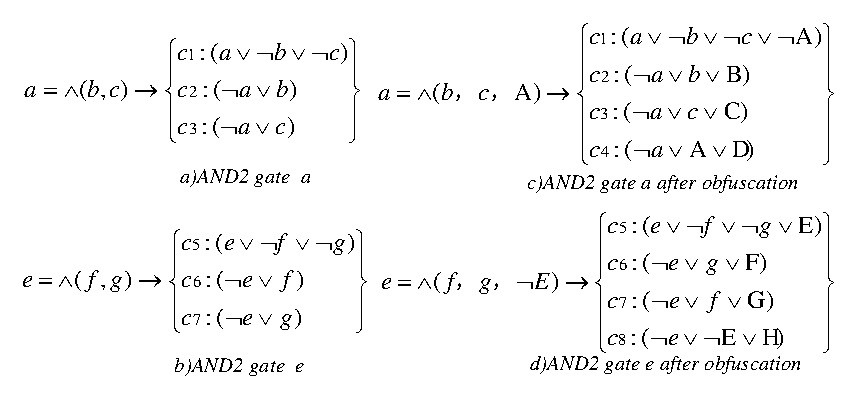
\includegraphics[width=8.2cm]{AND2-2}
%\caption{CNF signature of $a$ and $e$ before and after obfuscation}
%\label{fig_beforeafter}
%\end{figure}
%
%%Figure \ref{fig_beforeafter}a) and \ref{fig_beforeafter}b) shows the CNF signature and hyper-graph of two AND2 gate $a$ and $e$.
%%While their CNF signature and hypergraph after obfuscating are shown in Figure \ref{fig_beforeafter}c) and \ref{fig_beforeafter}d).
%Figure \ref{fig_beforeafter}a) and \ref{fig_beforeafter}b) shows the CNF signatures of two AND2 gates $a$ and $e$,
%while their CNF signatures after obfuscation are shown in Figure \ref{fig_beforeafter}c) and \ref{fig_beforeafter}d).
%
%There are three types of changes:
%\begin{enumerate}
% \item
% The length of key clauses $c_1$ and $c_5$ are changed from 3 to 4,
%this defeats structure detection techniques \upcite{csFu} based on key clause oriented pattern matching;
% \item
%CNF signatures of $a$ (characteristic clauses $c_1$-$c_3$) and $e$ (characteristic clauses $c_5$-$c_7$) are changed into different forms,
%and there are new clauses added in formula, such as $c_4$ and $c_8$,
%This defeats structure detection techniques\upcite{csRoy} based on sub-graph isomorphic;
%\item
% By inserting proper literals in key clauses and generating new clause,
% CNF signature of gate $a$ is changed from AND2 to AND3,
%shown in Figure \ref{fig_beforeafter}a) and \ref{fig_beforeafter}c).
%Husk variable $A$,
%which becomes an input variable of gate AND3,
%is indistinguishable with $b$ and $c$,
%which are original input variables of AND2.
%This makes it impossible to distinguish gates AND2 and AND3.
%\end{enumerate}

通过增加冗余的文字和子句,
OBFUSCATOR可以将CNF公式中的标记改变为另一合法标记.
在混淆之后,原始的CNF公式就被转化为混有噪音电路的另一个公式。
由于混淆后的的CNF公式被外包作为SAT求解器的输入,
原始CNF公式中的电路结构就并不再直接暴露给潜在的攻击者.

\begin{figure}[b]
\centering
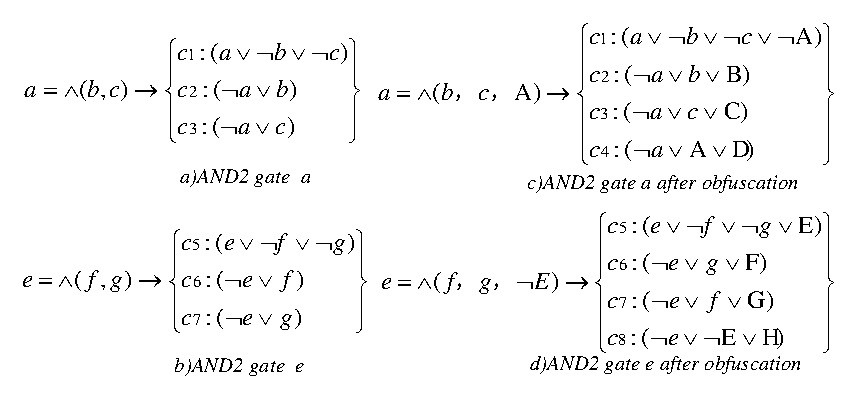
\includegraphics[width=8.2cm]{AND2-2}
\caption{混淆前后门$a$和门$e$的CNF标记}
%\caption{CNF signature of $a$ and $e$ before and after obfuscation}
\label{fig_beforeafter}
\end{figure}

%Figure \ref{fig_beforeafter}a) and \ref{fig_beforeafter}b) shows the CNF signature and hyper-graph of two AND2 gate $a$ and $e$.
%While their CNF signature and hypergraph after obfuscating are shown in Figure \ref{fig_beforeafter}c) and \ref{fig_beforeafter}d).
图\ref{fig_beforeafter}a)和\ref{fig_beforeafter}b)给出了两个AND2门$a$和$e$CNF标记,
混淆后的标记显示在图\ref{fig_beforeafter}c)和\ref{fig_beforeafter}d)中.

有三种改变
\begin{enumerate}
 \item
 关键子句$c_1$和$c_5$ 的长度由3变为4,
基于关键子句模式匹配的电路结构探测算法\upcite{csFu}将不再有效;
 \item
$a$的特征子句$c_1$-$c_3$)以及$e$的特征子句$c_5$-$c_7$变为了不同的形式,
并且有新的子句加入了公式如$c_4$和$c_8$,
基于标记子图同构的电路结构检测算法\upcite{csRoy}将不再有效;
\item
 通过加入合适的新文字以及构造新的子句,
 门$a$ 的CNF标记从AND2变为了AND3,
如图\ref{fig_beforeafter}a)和\ref{fig_beforeafter}c)。
Husk文字$A$,
成为了新生成的AND3门的一个输入,
并且与原始AND2门的输入$b$和$c$不可区分。
这也使得区分混淆后AND2和真实AND3变得不再可能.
\end{enumerate}
%
%\subsubsection{Output Camouflage by over-approximating solution space}
\subsubsection{输出数据隐藏}
根据\ref{SSOtheorem},
在SSO混淆之后解空间为原解空间的上估计.
这也就意味着,SAT求解器都无法确切知道真实的解。
首先,他们无法区分原始公式的变量和Husk公式的变量,而Husk公式的变量的赋值对验证毫无意义。
其次,他们无法确认一个可满足解也意味着原始SAT问题也是可满足,因为混淆会引入假解。
通过解空间上估计,我们把一个Rare Events转变为了一个Camouflaged Rare Events,这也是文献\upcite{HV-grid}曾经期待的事情。

\subsection{算法复杂性分析}
\subsubsection{混淆算法的复杂性}
%Obfuscation is implemented in Algorithm \ref{algo_obs}.
%The main procedure of Algorithm \ref{algo_obs} consists only one layer of loop,
%but one of it sub-procedure $\mathbf{mark}$ (Algorithm \ref{algo_mark}) consists 4 layers of loop,
%and the runtimes of the 2 inner loops are bounded by length of clauses.
%So the complexity of the obfuscation algorithm is $O(n^2)$.
算法\ref{algo_obs}实现了混淆,其中主程序仅仅包含一层循环,
但是其中一个子程序$\mathbf{mark}$(算法\ref{algo_mark})包含了4层循环,
由于两层内循环的上界为子句长度,因此混淆算法复杂性为$O(n^2)$。
\subsubsection{解恢复算法的复杂性}
%Solution recovery is implemented in  Algorithm \ref{algo_map},
%which only consists one layer of loop,
%its complexity is $O(n)$.
%According to Theorem \ref{SSOtheorem}, result from SAT solver may consist false solution,
%so Algorithm \ref{algo_map} may be run more than one time to get correct solution.
%Since Algorithm \ref{algo_map} is of linear complexity,
%it incurs minor impact on performance of SAT Solving.
解恢复在算法\ref{algo_map}中实现,
由于仅仅包含一层循环,算法复杂度为$O(n)$.
根据定理\ref{SSOtheorem}, 来自于SAT求解器的解可能包含假解,
因此为获得正确解,算法\ref{algo_map}可能会运行不只一次.
由于算法\ref{algo_map}为线性复杂度,
带给整个求解过程的开销较小.
%\section{Related work}
%\textbf{Secure Computation Outsourcing based on encryption:}
%R. Gennaro et al.\upcite{R.Gennaro} presented the concept of verifiable computation scheme,
%which shows the secure computation outsourcing is viable in theory.
%But the extremely high complexity of FHE operation and the pessimistic circuit sizes make it impractical.
%Zvika et al.\upcite{OBfuscationd-CNFs} constructed an obfuscated program for d-CNFs that preserves its functionality without revealing anything else.
%The construction is based on a generic multi-linear group model and graded encoding schemes,
%along with randomizing sub-assignments to enforce input consistency.
%But the scheme incurs large overhead caused by their fundamental primitives.
%
%\textbf{Secure Computation Outsourcing based on disguising:}
%For linear algebra algorithms,
%Atallah et al. \upcite{t19} multiplied data with random diagonal matrix before outsourcing.
%and recovered results by reversible matrix operations.
%Paper \upcite{t20} discussed secure outsourcing of numerical and scientific computation,
%by disguising with a set of problem dependent techniques.
%C.Wang\upcite{c.WANG} presented securely outsourcing linear programming(LP) in Cloud,
%by explicitly decomposing LP computation into public LP solvers and private data,
%and provide a practical mechanism which fulfills input/output privacy,
%cheating resilience, and efficiency.
%
%\textbf{Verifiable computation delegation:}
%Verifiable computation delegation is the technique to enable
%a computationally weak customer to verify the correctness of the delegated computation results
%from a powerful but untrusted server without investing too much resources.
%To prevent participants from keeping the rare events,
%Du. et al. \upcite{HV-grid} injected a number of chaff items into the workloads so as to confuse dishonest participants.
%Golle et al. \upcite{t32} proposed to insert some pre-computed results images of ringers
%into the computation workload to defeat untrusted or lazy workers.
%Szada et al. \upcite{t33} extended the ringer scheme and propose methods
%to deal with cheating detection.

%\section{相关工作}
%\textbf{基于加密的安全计算外包:}
%R. Gennaro等人\upcite{R.Gennaro}给出了可验证计算的策略,
%指出了安全计算外包的理论上可行性.
%但是同构加密操作的复杂性和悲观的电路尺寸使得还未能实际使用.
%Zvika等人\upcite{OBfuscationd-CNFs}构造了面向d-CNFs的混淆程序,用来保持函数功能的同时隐藏信息.
%他们的构造过程基于通用的多线性群模型以及坡度加密策略,以及随机的赋值以保证输入的一致性。
%他们的方法是面向通用的SAT问题,由于原语引入的开销较大。
%
%\textbf{基于伪装的安全计算外包:}
%对于线性代数算法,
%Atallah等人\upcite{t19}使用对角矩阵乘来伪装外包数据,并通过反向矩阵操作来恢复结果。
%文献\upcite{t20}讨论了通过特定问题相关技术来伪装数据,实现数值和科学计算的安全外包。
%C.Wang\upcite{c.WANG}给出了线性规划的安全外包方法,
%通过显示的将LP计算划分为公共的LP求解和私有数据,
%并且给出了实现输入输出隐私保护,欺骗防御的可行的机制.
%
%\textbf{可验证的计算代理:}
%可验证计算代理技术是指,一个计算能力弱的客户端可以较小的计算量来验证不可信服务器提供的计算结果正确性。
%Golle et al. \upcite{t32} 给出了插入预先计算结果到计算负载中,以便于防止不诚实以及懒惰的工人。
%Szada et al. \upcite{t33} 扩展了ringer策略并且给出了欺骗检测的方法.
%为了防止不可信的计算参与者持有计算结果,
%Du等人\upcite{HV-grid}将一定数量的chaff插入到工作集中以便于误导不诚实的参与者.

\section{实验评估}
%Algorithms presented in this paper are implemented in language $C$.
%The experiments is conducted on a laptop with Intel Core(TM) i7-3667U CPU @ 2.00GHz, 8GB RAM.
%
%We unroll circuits in ISCAS89 benchmark for 100 times and transform them into CNF formulas,
%and generate Husks formula with variables number $vn=675$ and clauses number $cn=2309$,
%and then obfuscate the CNF formula by transform 2 input gates into 3 input gates.
%We use MiniSat as solver.
%
%Table \ref{fig_exp} presents experiments result on benchmarks, meaning of parameters are listed below. \\
%$~~$\textbf{vn/cn}:variable and clause number of CNF formula.\\
%$~~$\textbf{Marked Gate}:number of gates being changed in obfuscation.\\
%$~~$\textbf{Solve Times}:SAT Solver time before and after obfuscation.\\
%$~~$\textbf{Obfuscation Times}:obfuscation time.\\
%$~~$\textbf{Map Time}:solution recovery time.
%
%Acccording to Algorithm \ref{algo_obs},
%Obfusaction time is up to number of gates being changed,
%while solution recovery time is up to size of CNF formula,
%experiments manifest the fact.
%% Detailed information are listed in columns of \textbf{Marked~Gate}, \textbf{Obfuscation Times} and \textbf{Map~Times}.
%
%As for Asymmetric Speedup\upcite{c.WANG}, for more than 60 \% of circuits, the value is more than 260\%,
%It indicates the necessity of outsourcing complex SAT solving.
%But for some small size circuits,
%Asymmetric Speedup is less than 1.
%Especially for circuit s3384,
%since the obfuscation takes lots of time to transform 139860 gates, Asymmetric Speedup is only 5.22\%.
%\begin{equation}
% Asymmetric~Speedup= \frac{Solving~Time}{Obfuscation~Times + Map~Time}
%\end{equation}
%
%The experiments also show that overhead of SAT solving time, incurred by obfuscation,
%are different among circuits.
%For more than 60 \% of circuits, overhead is less than 30\%; But for the other 40\% circuits, overhead exceed 100\%.
%
%These facts remind us at least two things:
%First, since  obfuscation time is up to gates being changed,
%delicate obfuscation algorithm which change less gates but still can mislead adversary should be studied.
%Second, since overhead on SAT solving incurred by obfuscation are different among circuit benchmarks,
%much more attention should be pay on the impact on solving time,  when designing obfuscation algorithm.
%\begin{figure}
%\centering
%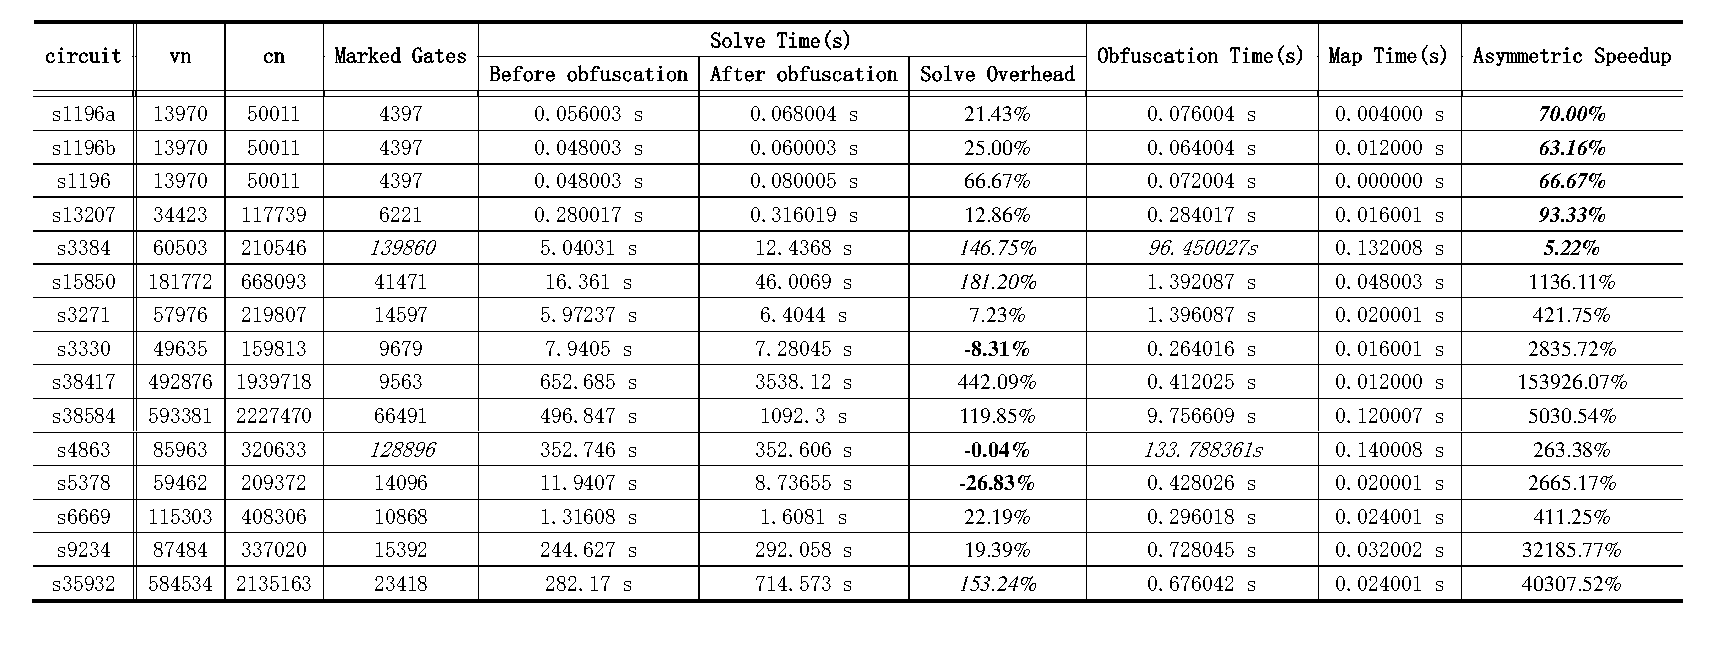
\includegraphics[width=16cm]{Experiment}
%\caption{Relationship between Runtime and Size of CNF formula}
%\label{fig_exp}
%\end{figure}
\subsection{实验设计}
本文给出的算法由C语言实现.
实验用机器的配置为Intel Core(TM) i7-3667U CPU @ 2.00GHz, 8GB RAM.

将ISCAS89测试集中的部分电路展开100次并编码为CNF公式,
产生的Husks公式包含了节点数和子句数为$vn=675$/$cn=2309$,
并且将原始公式中的2输入门转换为3输入门.
使用MiniSat作为求解器.
\subsection{实验结果分析}
表\ref{fig_exp}给出了实验结果,表中各个参数的意义如下所示。 \\
$~~$\textbf{vn/cn}:CNF 公式中的变量数和子句数.\\
$~~$\textbf{Marked Gate}:混淆过程中改变的门数.\\
$~~$\textbf{Solve Times}:混淆前后的SAT求解时间.\\
$~~$\textbf{Obfuscation Times}:混淆时间.\\
$~~$\textbf{Map Time}:解恢复时间.

根据算法\ref{algo_obs},
混淆时间取决于改变的门数,
解恢复时间取决于CNF公式的尺寸,
实验表明了这一事实.
% Detailed information are listed in columns of \textbf{Marked~Gate}, \textbf{Obfuscation Times} and \textbf{Map~Times}.

就异构加速比( Asymmetric~Speedup)\upcite{c.WANG}而言,60\%的电路, 值超过了260\%,
这表明了外包复杂SAT求解函数的必要性.
某些尺寸较小的电路B,异构加速比小于1.
特别是对于电路s3384,
由于混淆花费了大量的时间,转换了139860个门,使得异构加速比仅为5.22\%.
\begin{equation}
 Asymmetric~Speedup= \frac{Solving~Time}{Obfuscation~Times + Map~Time}
\end{equation}

实验也显示出SAT求解的开销,不同的电路具有不同的表现。
60 \% 以上的电路,开销小于30\%;而40\%电路,开销超过了100\%.

这些事实提醒我们两件事情:
首先,混淆时间取决于被改变的门数,
需要研究更加精巧的混淆算法以改变较少的门的情况下仍然可以迷惑攻击者.
第二, 由于混淆引入的SAT求解开销,因电路而异,在设计混淆算法时,需要考虑修改后结构对求解时间的影响。

\begin{table*}
\caption{不同类型电路的CNF公式的运行时间}
%\caption{Runtime of CNF formula generated from different Circuit}
\centering
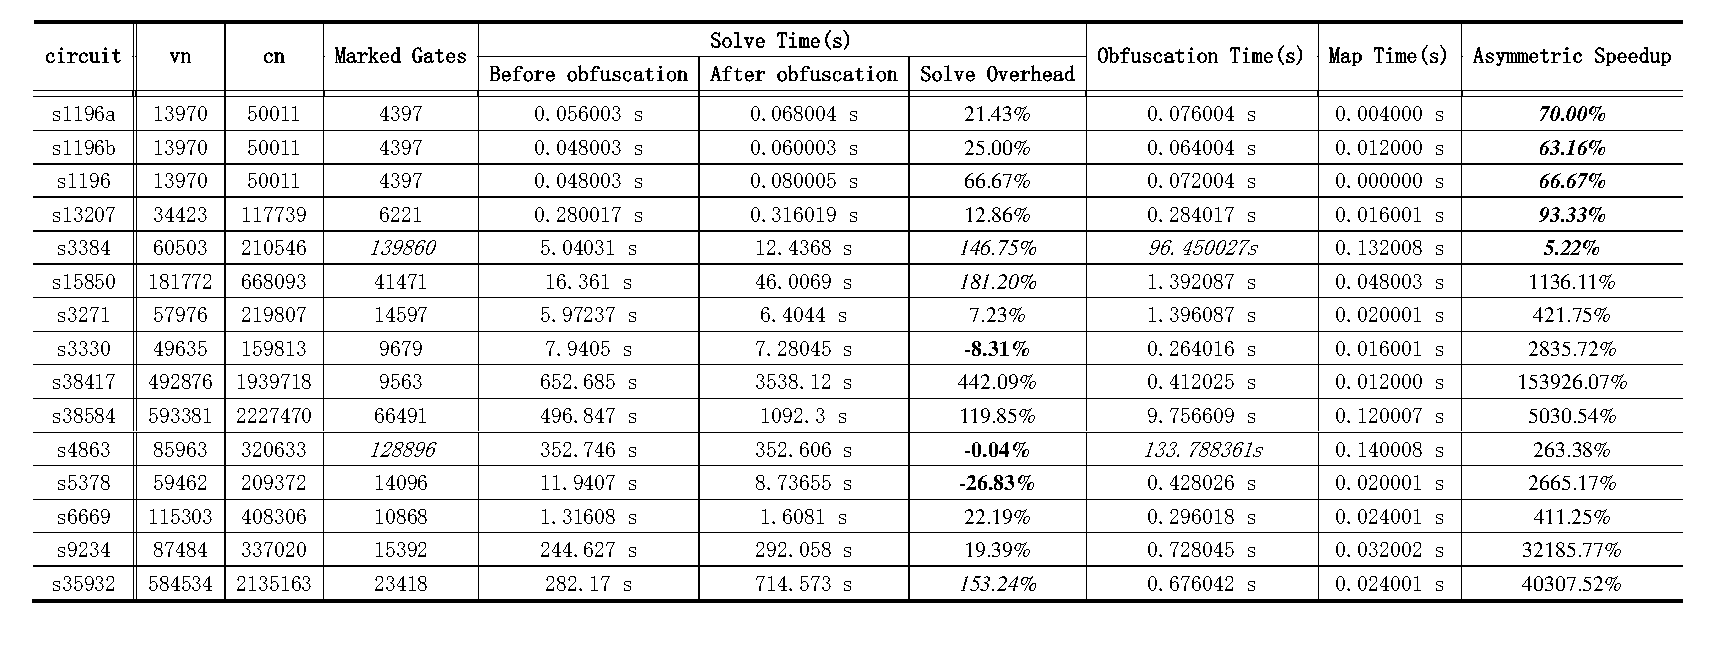
\includegraphics[width=14.2cm]{Experiment}
\label{fig_exp}
\end{table*}%
%
%\section{Conclusion}
%This paper proposes a circuit aware  CNF obfuscation algorithm,
%that can prevent the confidential information from being recovered by adversary,
%when outsourcing SAT problem in Cloud or grid.
%Theoretical analysis and experimental results show that algorithms can significantly change structure of CNF formula,
%with polynomial complexity and without narrowing down its solution space.
\section{结论}
本文给出了电路结构感知且解空间加噪的CNF混淆算法,可防止在SAT问题外包计算时,CNF公式中的电路结构以及解被窃取。
理论分析和实验表明,算法可以有效的改变结构,同时还不会缩减CNF公式的解空间。
